\documentclass[12pt, numbers=noenddot]{scrreprt} %use komascript instead of just article
\setkomafont{disposition}{\normalcolor\bfseries} %use the standard article look
\usepackage[margin=1in]{geometry}
\usepackage{graphicx}
\usepackage{cite}
\usepackage{amsthm, amsmath, amssymb}
\usepackage{setspace}\onehalfspacing
%\usepackage{setspace}\doublespacing
\usepackage[loose,nice]{units} %replace "nice" by "ugly" for units in upright fractions
\usepackage{parskip} % dont't need to du double backslash for linebreak
\usepackage[linktocpage=true]{hyperref}
\usepackage{tabularx} % in the preamble

\usepackage{hyperref}
\hypersetup{
    colorlinks=true,
    linkcolor=blue,
    filecolor=magenta,      
    urlcolor=cyan,
}
 
\urlstyle{same}



\title{The Data Engineering Cookbook}
\subtitle{Mastering The Plumbing Of Data Science}
\author{Andreas Kretz}
\date{\today\\v1.2}

\begin{document}
\maketitle

 %\begin{abstract}
%Purpous of this document and its conclusion
%\end{abstract}

\pagebreak

\setcounter{tocdepth}{3}
\tableofcontents

\pagebreak

\part{Introduction}
\chapter{How To Use This Cookbook}
What do you actually need to learn to become an awesome data engineer?
Look no further, you'll find it here. 

If you are looking for AI algorithms and such data scientist things, this book is not for you.

\textbf{How to use this document:} \\ 
First of all, this is not a training! This cookbook is a collection of skills that I value highly in my daily work as a data engineer. It's intended to be a starting point for you to find the topics to look into and become a data engineer.

You are going to find \textbf{\textit{three types of content}} in this book that will help you understand each topic: Articles I wrote, relevant links to my podcast episodes (video \& audio) and links to helpful websites I like. 

\textbf{This book is a work in progress!} \\
As you can see, this book is not finished. I'm constantly adding new stuff and doing videos for the topics. But obviously, because I do this as a hobby my time is limited. You can help making this book even better.

\textbf{Help make this book awesome!}\\
If you have some cool links or topics for the cookbook, please become a contributor on GitHub: \url{https://github.com/andkret/Cookbook}. Pull the repo, add them and create a pull request. Or join the discussion by opening Issues.
You can also write me an email any time to plumbersofdatascience@gmail.com. Tell me your thoughts, what you value, you think should be included, or correct where I am wrong.

\textbf{This Cookbook is and will always be free! }\\
I don't want to sell you this book, but please support what you like and join my Patreon: \url{https://www.patreon.com/plumbersofds} 

Check out this podcast episode where I talk in detail why I decided to share all this information for free: 
\href{https://youtu.be/k1bS5aSPos8}{\#079 Trying to stay true to myself and making the cookbook public on GitHub}

\pagebreak

\chapter{Data Engineer vs Data Scientists}

\section{Data Scientist}
Data scientists aren’t like every other scientist.

Data scientists do not wear white coats or work in high tech labs full of science fiction movie equipment. They work in offices just like you and me.

What differs them from most of us is that they are the math experts. They use linear algebra and multivariable calculus to create new insight from existing data.

How exactly does this insight look?

Here’s an example:

An industrial company produces a lot of products that need to be tested before shipping.

Usually such tests take a lot of time because there are hundreds of things to be tested. All to make sure that your product is not broken.

Wouldn’t it be great to know early if a test fails ten steps down the line? If you knew that you could skip the other tests and just trash the product or repair it.

That’s exactly where a data scientist can help you, big-time. This field is called predictive analytics and the technique of choice is machine learning.

Machine what? Learning?

Yes, machine learning, it works like this:

You feed an algorithm with measurement data.
It generates a model and optimises it based on the data you fed it with. That model basically represents a pattern of how your data is looking
You show that model new data and the model will tell you if the data still represents the data you have trained it with.
This technique can also be used for predicting machine failure in advance with machine learning. Of course the whole process is not that simple.

The actual process of training and applying a model is not that hard. A lot of work for the data scientist is to figure out how to pre-process the data that gets fed to the algorithms.

Because to train a algorithm you need useful data. If you use any data for the training the produced model will be very unreliable.

A unreliable model for predicting machine failure would tell you that your machine is damaged even if it is not. Or even worse: It would tell you the machine is ok even when there is an malfunction.

Model outputs are very abstract. You also need to post-process the model outputs to receive health values from 0 to 100.

\begin{figure}[htbp]
  \centering
     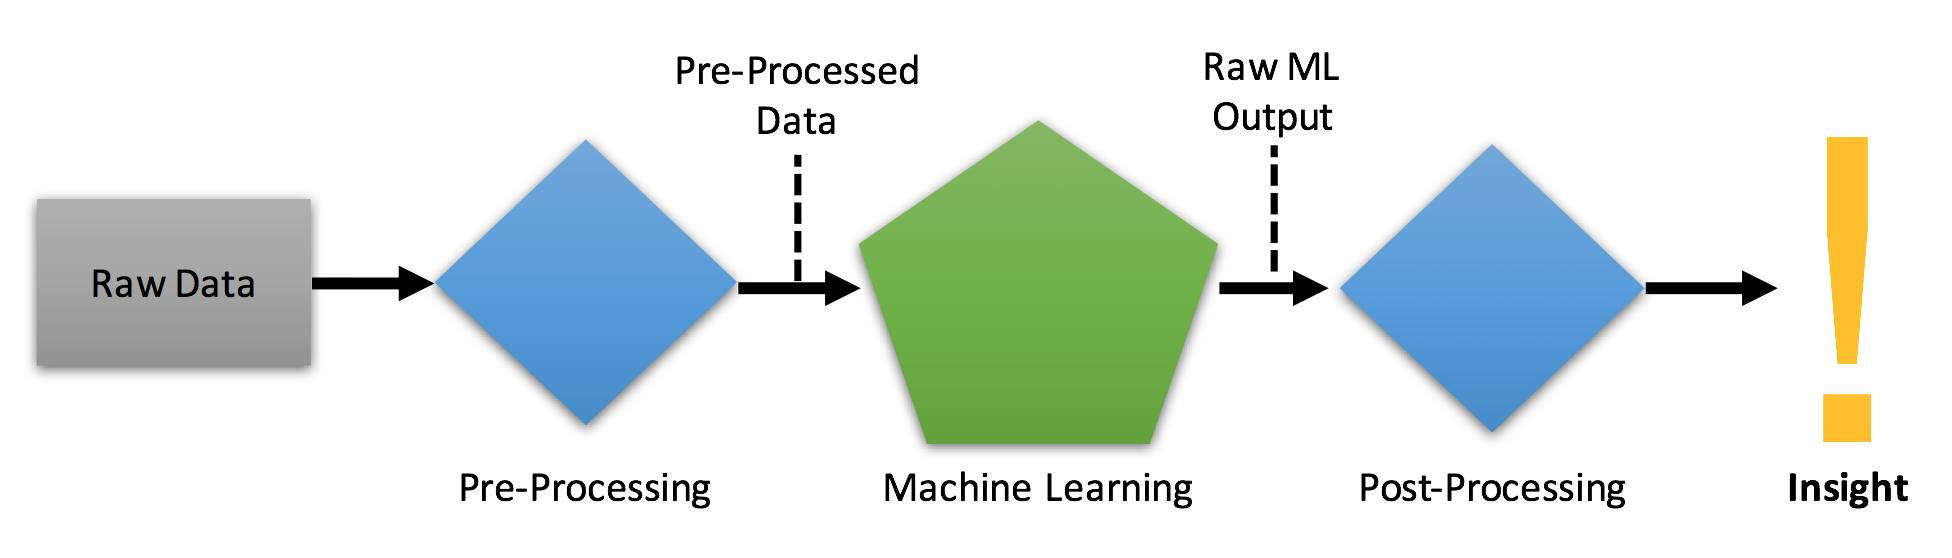
\includegraphics[width=0.9\textwidth]{images/Machine-Learning-Pipeline}
  \caption{The Machine Learning Pipeline}
  \label{fig:Bild1}
\end{figure}

\section{Data Engineer}
Data Engineers are the link between the management’s big data strategy and the data scientists that need to work with data.

What they do is building the platforms that enable data scientists to do their magic.

These platforms are usually used in five different ways:

\begin{itemize}
\item  Data ingestion and storage of large amounts of data
\item Algorithm creation by data scientists
\item Automation of the data scientist’s machine learning models and algorithms for production use
\item Data visualisation for employees and customers
\item  Most of the time these guys start as traditional solution architects for systems that involve SQL databases, web servers, SAP installations and other “standard” systems.
\end{itemize}

But to create big data platforms the engineer needs to be an expert in specifying, setting up and maintaining big data technologies like: Hadoop, Spark, HBase, Cassandra, MongoDB, Kafka, Redis and more.

What they also need is experience on how to deploy systems on cloud infrastructure like at Amazon or Google or on premise hardware.

\section{Who Companies Need}
For a good company it is absolutely important to get well trained data engineers and data scientists.

Think of the data scientist as the professional race car driver. A fit athlete with talent and driving skills like you have never seen.

What he needs to win races is someone who will provide him the perfect race car to drive. That’s what the solution architect is for.

Like the driver and his team the data scientist and the data engineer need to work closely together. They need to know the different big data tools Inside and out.

That's why companies are looking for people with Spark experience. It is a common ground between both that drives innovation.

Spark gives data scientists the tools to do analytics and helps engineers to bring the data scientist’s algorithms into production.

After all, those two decide how good the data platform is, how good the analytics insight is and how fast the whole system gets into a production ready state.


\part{Basic Data Engineering Skills}

\chapter{Learn To Code}

Why this is important: Without coding you cannot do much in data engineering. I cannot count the number of times I needed a quick Java hack.

The possibilities are endless:

\begin{itemize}
\item Writing or quickly getting some data out of a SQL DB
\item Testing to produce messages to a Kafka topic
\item Understanding Source code of a Java Webservice
\item Reading counter statistics out of a HBase key value store
\end{itemize}
So, which language do I recommend then?

I highly recommend Java. It’s everywhere!

When you are getting into data processing with Spark you should use Scala. But, after learning Java this is easy to do.

Also Python is a great choice. It is super versatile.

Personally however, I am not that big into Python. But I am going to look into it

Where to Learn?
There’s a Java Course on Udemy you could look at: https://www.udemy.com/java-programming-tutorial-for-beginners

\begin{itemize}
\item OOP Object oriented programming
\item What are Unit tests to make sure what you code is working
\item Functional Programming
\item How to use build management tools like Maven
\item Resilient testing (?)
\end{itemize}
I talked about the importance of learning by doing in this podcast: 
\url{https://anchor.fm/andreaskayy/episodes/Learning-By-Doing-Is-The-Best-Thing-Ever---PoDS-035-e25g44}

\chapter{Get Familiar With Git}
Why this is important: One of the major problems with coding is to keep track of changes. It is also almost impossible to maintain a program you have multiple versions of.

Another is the topic of collaboration and documentation. Which is super Important.

Let’s say you work on a Spark application and your colleagues need to make changes while you are on holiday. Without some code management they are in huge trouble:

Where is the code? What have you changed last? Where is the documentation? How do we mark what we have changed?

But if you put your code on GitHub your colleagues can find your code. They can understand it through your documentation (please also have in-line comments)

Developers can pull your code, make a new branch and do the changes. After your holiday you can inspect what they have done and merge it with your original code. and you end up having only one application

Where to learn:
Check out the GitHub Guides page where you can learn all the basics: https://guides.github.com/introduction/flow/

This great GitHub commands cheat sheet saved my butt multiple times: https://www.atlassian.com/git/tutorials/atlassian-git-cheatsheet

Also look into:
\begin{itemize}
\item Pull
\item Push
\item Branching
\item Forking
\end{itemize}


\chapter{Agile Development  -- available}
Agility, the ability to adapt quickly to changing circumstances.

These days everyone wants to be agile. Big or small company people are looking for the “startup mentality”.

Many think it’s the corporate culture. Others think it’s the process how we create things that matters.

In this article I am going to talk about agility and self-reliance. About how you can incorporate agility in your professional career.

\section{Why is agile so important?}
Historically development is practiced as a hard defined process. You think of something, specify it, have it developed and then built in mass production.

It’s a bit of an arrogant process. You assume that you already know exactly what a customer wants. Or how a product has to look and how everything works out.

The problem is that the world does not work this way!

Often times the circumstances change because of internal factors.

Sometimes things just do not work out as planned or stuff is harder than you think.

You need to adapt.

Other times you find out that you build something customers do not like and need to be changed.

You need to adapt.

That’s why people jump on the Scrum train. Because Scrum is the definition of agile development, right?

\section{Agile rules I learned over the years -- available}

\subsection{Is the method making a difference?}
Yes, Scrum or Google’s OKR can help to be more agile. The secret to being agile however, is not only how you create.

What makes me cringe is people try to tell you that being agile starts in your head. So, the problem is you?

No!

The biggest lesson I have learned over the past years is this: Agility goes down the drain when you outsource work.

\subsection{The problem with outsourcing}
I know on paper outsourcing seems like a no brainer: Development costs against the fixed costs.

It is expensive to bind existing resources on a task. It is even more expensive if you need to hire new employees.

The problem with outsourcing is that you pay someone to build stuff for you.

It does not matter who you pay to do something for you. He needs to make money.

His agenda will be to spend as less time as possible on your work. That is why outsourcing requires contracts, detailed specifications, timetables and delivery dates.

He doesn’t want to spend additional time on a project, only because you want changes in the middle. Every unplanned change costs him time and therefore money.

If so, you need to make another detailed specification and a contract change.

He is not going to put his mind into improving the product while developing. Firstly because he does not have the big picture. Secondly because he does not want to.

He is doing as he is told.

Who can blame him? If I was the subcontractor I would do exactly the same!

Does this sound agile to you?

\subsection{Knowledge is king: A lesson from Elon Musk}
Doing everything in house, that’s why startups are so productive. No time is wasted on waiting for someone else.

If something does not work, or needs to be changed, there is someone in the team who can do it right away.                        .

One very prominent example who follows this strategy is Elon Musk.

Tesla’s Gigafactories are designed to get raw materials in on one side and spit out cars on the other. Why do you think Tesla is building Gigafactories who cost a lot of money?

Why is SpaceX building its one space engines? Clearly there are other, older, companies who could do that for them.

Why is Elon building tunnel boring machines at his new boring company?

At first glance this makes no sense!

\subsection{How you really can be agile}
If you look closer it all comes down to control and knowledge. You, your team, your company, needs to as much as possible on your own. Self-reliance is king.

Build up your knowledge and therefore the teams knowledge. When you have the ability to do everything yourself, you are in full control.

You can build electric cars, rocket engines or bore tunnels.

Don’t largely rely on others and be confident to just do stuff on your own.

Dream big and JUST DO IT!

PS. Don’t get me wrong. You can still outsource work. Just do it in a smart way by outsourcing small independent parts.

\section{Agile Frameworks}
\subsection{Scrum}

There's a interesting Scrum Medium publication with a lot of details about Scrum: \url{https://medium.com/serious-scrum}

Also this scrum guide webpage has good infos about Scrum: \url{https://www.scrumguides.org/scrum-guide.html}

\subsection{OKR}

I personally love OKR, been doing it for years. Especially for smaller teams OKR is great. You don't have a lot of overhead and get work done.
It helps you stay focused and look at the bigger picture. 

I recommend to do a sync meeting every Monday. There you talk about what happened last week and what you are going to work on this week.

I talked about this in this Podcast: \url{https://anchor.fm/andreaskayy/embed/episodes/Agile-Development-Is-Important-But-Please-Dont-Do-Scrum--PoDS-041-e2e2j4}

This is also this awesome 1,5 hours Startup guide from Google: \url{https://youtu.be/mJB83EZtAjc} I really love this video, I rewatched it multiple times.

 \chapter{Learn how a Computer Works}

\section{CPU,RAM,GPU,HDD}

\section{Differences between PCs and Servers}

I talked about computer hardware and GPU processing in this podcast: \url{https://anchor.fm/andreaskayy/embed/episodes/Why-the-hardware-and-the-GPU-is-super-important--PoDS-030-e23rig}

\chapter{Computer Networking - Data Transmission}

\section{OSI Model}

The OSI Model describes how data is flowing through the network. It consists of layers starting from physical layers, basically how the data is transmitted over the line or optic fiber. 

Cisco page that shows the layers of the OSI model and how it works: \url{https://learningnetwork.cisco.com/docs/DOC-30382}
 
Check out this page: \url{https://www.studytonight.com/computer-networks/complete-osi-model}

The Wikipedia page is also very good: \url{https://en.wikipedia.org/wiki/OSI_model}

\paragraph{Which protocol lives on which layer?} Check out this network protocol map. Unfortunately it is really hard to find it theses days:
\url{https://www.blackmagicboxes.com/wp-content/uploads/2016/12/Network-Protocols-Map-Poster.jpg}

\section{IP Subnetting}

Check out this IP Adress and Subnet guide from Cisco: \url{https://www.cisco.com/c/en/us/support/docs/ip/routing-information-protocol-rip/13788-3.html}

A calculator for Subnets: \url{https://www.calculator.net/ip-subnet-calculator.html}

\section{Switch, Level 3 Switch}

\section{Router}

\section{Firewalls}

I talked about Network Infrastructure and Techniques in this podcast: \url{https://anchor.fm/andreaskayy/embed/episodes/IT-Networking-Infrastructure-and-Linux-031-PoDS-e242bh}

\chapter{Security and Privacy}
\section{SSL Public \& Private Key Certificates}

\section{What is a certificate authority}

\section{JSON Web Tokens}

Link to the Wiki page: \url{https://en.wikipedia.org/wiki/JSON_Web_Token}

\section{GDPR regulations}

\section{Privacy by design}

\chapter{Linux}

Linux is very important to learn, at least the basics. Most Big Data tools or NoSQL databases are running on Linux. 

From time to time you need to modify stuff through the operation system. Especially if you run a infrastructure as a service solution like Cloudera CDH, Hortonworks or a MapR Hadoop distribution

\section{OS Basics}

\section{Shell scripting}

\section{Cron jobs}

Cron jobs are super important to automate simple processes or jobs in Linux. You need this here and there I promise.
Check out this three guides:

\url{https://linuxconfig.org/linux-crontab-reference-guide}

\url{https://www.ostechnix.com/a-beginners-guide-to-cron-jobs/}

And of course Wikipedia, which is surprisingly good: \url{https://en.wikipedia.org/wiki/Cron}

Pro tip: Don't forget to end your cron files with an empty line or a comment, otherwise it will not work.

\section{Packet management}
Linux Tips are the second part of this podcast: \url{https://anchor.fm/andreaskayy/embed/episodes/IT-Networking-Infrastructure-and-Linux-031-PoDS-e242bh}

\chapter{The Cloud}
\section{IaaS vs PaaS vs SaaS}

Check out this Podcast it will help you understand where's the difference and how to decide on what you are going to use.

\begin{table}[h]
\begin{tabular}{ll}
\hline
\multicolumn{2}{l}{\textbf{Podcast Episode:} \#082 Reading Tweets With Apache Nifi \& IaaS vs PaaS vs SaaS} \\ \hline
\multicolumn{2}{p{15cm}}{In this episode we are talking about the differences between infrastructure as a service, platform as a service and application as a service. Then we install the Nifi docker container and look into how we can extract the twitter data.}         \\ \hline
\multicolumn{1}{l|}{Audio}     & \href{https://anchor.fm/andreaskayy/episodes/082-Reading-Tweets-With-Apache-Nifi--IaaS-vs-PaaS-vs-SaaS-e45j50}{Click here to listen}   \\
\multicolumn{1}{l|}{Youtube}   & \href{https://youtu.be/pWuT4UAocUY}{Click here to watch}   \\ \hline
\end{tabular}
\end{table}


\section{AWS,Azure, IBM, Google Cloud basics}
\section{cloud vs on premise}
\section{up \& downsides}
\section{Security}

Listen to a few thoughts about the cloud in this podcast: \url{https://anchor.fm/andreaskayy/embed/episodes/Dont-Be-Arrogant-The-Cloud-is-Safer-Then-Your-On-Premise-e16k9s}

\chapter{Security Zone Design}
\section{How to secure a multi layered application}
(UI in different zone then SQL DB)

\section{Cluster security with Kerberos}

I talked about security zone design and lambda architecture in this podcast: \url{https://anchor.fm/andreaskayy/embed/episodes/How-to-Design-Security-Zones-and-Lambda-Architecture--PoDS-032-e248q2}

\section{Kerberos Tickets}

\chapter{Stream Processing}
\section{Three methods of streaming | available}

In stream processing sometimes it is ok to drop messages, other times it is not. Sometimes it is fine to process a message multiple times, other times that needs to be avoided like hell.

Today’s topic are the different methods of streaming: At most once, at least once and exactly once.

What this means and why it is so important to keep them in mind when creating a solution. That is what you will find out in this article.

\section{At Least Once}

At least once, means a message gets processed in the system once or multiple times. So with at least once it’s not possible that a message gets into the system and is not getting processed.

It’s not getting dropped or lost somewhere in the system.

One example where at least once processing can be used is when you think about a fleet management of cars. You get GPS data from cars and that GPS data is transmitted with a timestamp and the GPS coordinates.

It’s important that you get the GPS data at least once, so you know where the car is. If you’re processing this data multiple times, it always has the the timestamp with it.

Because of that it does not matter that it gets processed multiple times, because of the timestamp. Or that it would be stored multiple times, because it would just override the existing one.

\section{At Most Once}

The second streaming method is at most once. At most once means that it’s okay to drop some information, to drop some messages.

But it’s important that a message is only only processed once as a maximum.

A example for this is event processing. Some event is happening and that event is not important enough, so it can be dropped. It doesn’t have any consequences when it gets dropped.

But when that event happens it’s important that it does not get processed multiple times. Then it would look as if the event happened five or six times instead of only one.

Think about engine misfires. If it happens once, no big deal. But if the system tells you it happens a lot you will think you have a problem with your engine.

\section{Exactly Once}

Another thing is exactly once, this means it’s not okay to drop data, it’s not okay to lose data and it’s also not okay to process one message what data said multiple times

A example for this is for instance banking. When you think about credit card transactions it’s not okay to drop a transaction.

When dropped your payment is not going through. It’s also not okay to have a transaction processed multiple times, because then you are paying multiple times.

\section{Check The Tools!}

All of this sounds very simple and logical. What kind of processing is done has to be a requirement for your use case.

It needs to be thought about in the design process, because not every tool is supporting all three methods. Very often you need to code your application very differently based on the streaming method.

Especially exactly once is very hard to do.

So, the tool of data processing needs to be chosen based on if you need exactly once, at least once or if you need at most once.

\chapter{Big Data}
\section{What is big data and where is the difference to data science and data analytics?}
I talked about the difference in this podcast: https://anchor.fm/andreaskayy/embed/episodes/BI-vs-Data-Science-vs-Big-Data-e199hq

\section{The 4Vs of Big Data | available}

It is a complete misconception. Volume is only one part of the often called four V’s of big data: Volume, velocity, variety and veracity.

\textbf{Volume} is about the size. How much data you have.

\textbf{Velocity} is about the speed of how fast the data is getting to you.

How much data is in a specific time needs to get processed or is coming into the system. This is where the whole concept of streaming data and real-time processing comes in to play.

\textbf{Variety} is the third one. It means, that the data is very different. That you have very different types of data structures.

Like CSV files, PDFs that you have stuff in XML. That you have JSON logfiles, or that you have data in some kind of a key value store.

It’s about the variety of data types from different sources that you basically want to join together. All to make an analysis based on that data.

\textbf{Veracity} is fourth and this is a very very difficult one. The issue with big data is, that it is very unreliable.

You cannot really trust the data. Especially when you’re coming from the IoT, the Internet of Things side. Devices use sensors for measurement of temperature, pressure, acceleration and so on.

You cannot always be hundred percent sure that the actual measurement is right.

When you have data that is from for instance SAP and it contains data that is created by hand you also have problems. As you know we humans are bad at inputting stuff.

Everybody articulates different. We make mistakes, down to the spelling and that can be a very difficult issue for analytics.


I talked about the 4Vs in this podcast: https://anchor.fm/andreaskayy/embed/episodes/4-Vs-Of-Big-Data-Are-Enough-e1h2ra

\section{Why Big Data? | available}

What I always emphasize is the four V’s are quite nice. They give you a general direction.

There is a much more important issue: Catastrophic Success.

What I mean by catastrophic success is, that your project, your startup or your platform has more growth that you anticipated. Exponential growth is what everybody is looking for.

Because with exponential growth there is the money. It starts small and gets very big very fast. The classic hockey stick curve:

1,2,4,8,16,32,64,128,256,512,1024,2048,4096,8192,16384….BOOM!

Think about it. It starts small and quite slow, but gets very big very fast.

You get a lot of users or customers who are paying money to use your service, the platform or whatever. If you have a system that is not equipped to scale and process the data the whole system breaks down.

That’s catastrophic success. You are so successful and grow so fast that you cannot fulfill the demand anymore. And so you fail and it’s all over.

It’s now like you just can make that up while you go. That you can foresee in a few months or weeks the current system doesn’t work anymore.

\subsection{Planning is Everything}

It’s all happens very very fast and you cannot react anymore. There’s a necessary type of planning and analyzing the potential of your business case necessary.

Then you need to decide if you actually have big data or not.

You need to decide if you use big data tools. This means when you conceptualize the whole infrastructure it might look ridiculous to actually focus on big data tools.

But in the long run it will help you a lot. Good planning will get a lot of problems out of the way, especially if you think about streaming data and real-time analytics.

\subsection{The Problem With ETL}
A typical old-school platform deployment would look like the picture below. Devices use a data API to upload data that gets stored in a SQL database. An external analytics tool is querying data and uploading the results back to the SQL db. Users then use the user interface to display data stored in the database.

\begin{figure}[htbp]
  \centering
     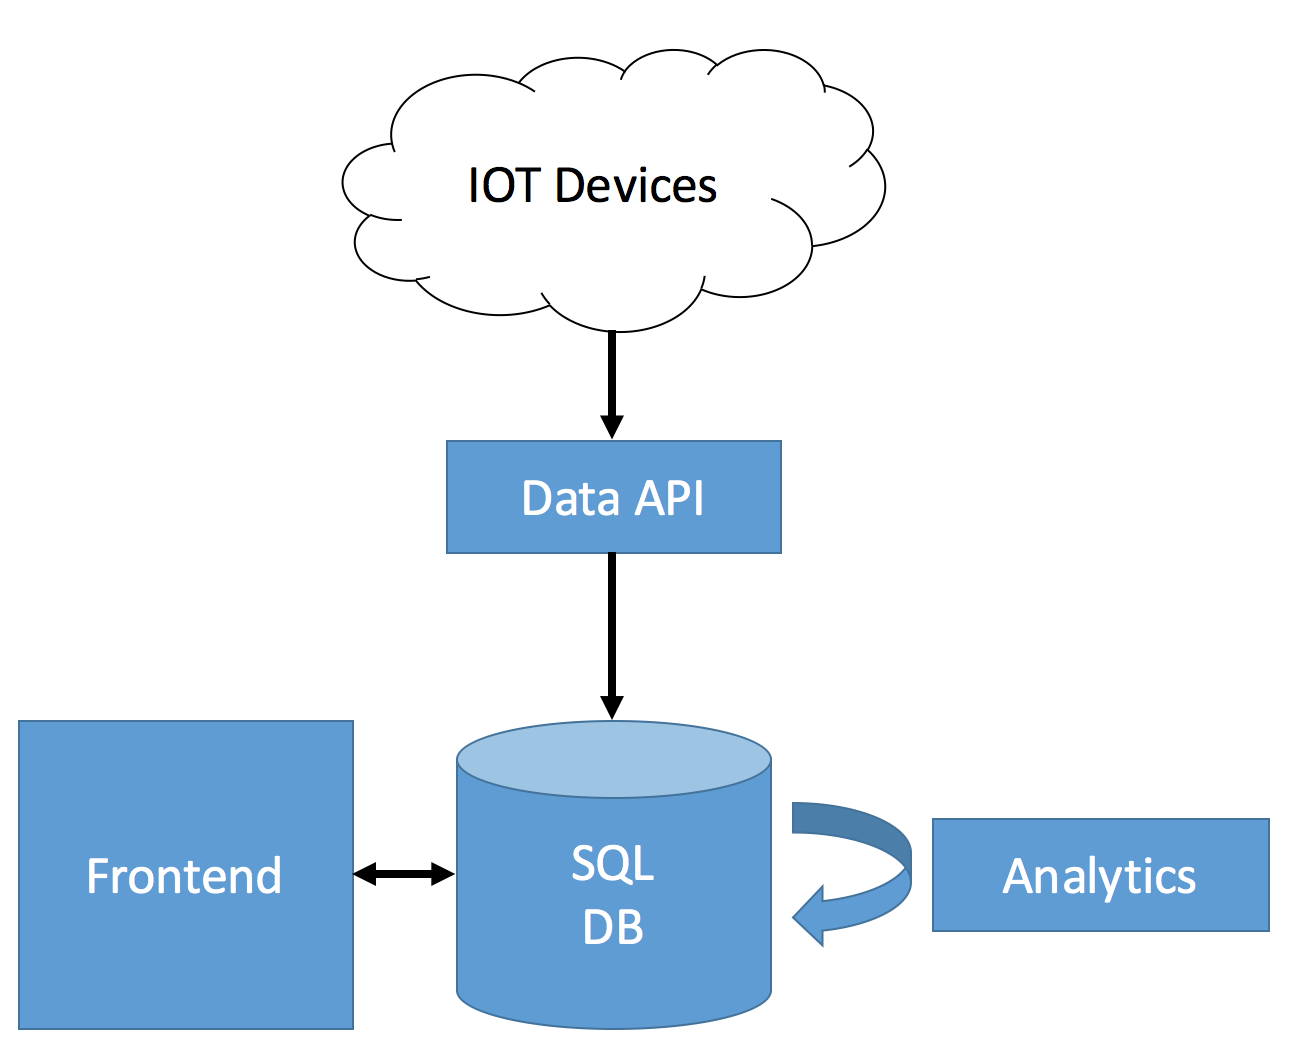
\includegraphics[width=0.7\textwidth]{images/Common-SQL-Architecture}
  \caption{Common SQL Platform Architecture}
  \label{fig:Bild1}
\end{figure}

Now, when the front end queries data from the SQL database the following three steps happen:

The database extracts all the needed rows from the storage. Extracted data gets transformed, for instance sorted by timestamp or something a lot more complex.

The extracted and transformed data gets loaded to the destination (the user interface) for chart creation
With exploding amounts of stored data the ETL process starts being a real problem.

Analytics is working with large data sets, for instance whole days, weeks, months or more. Data sets are very big like 100GB or Terabytes. That means Billions or Trillions of rows.

This has the result that the ETL process for large data sets takes longer and longer. Very quickly the ETL performance gets so bad it won’t deliver results to analytics anymore.

A traditional solution to overcome these performance issues is trying to increase the performance of the database server. That’s what’s called scaling up.

\subsection{Scaling Up}
To scale up the system and therefore increase ETL speeds administrators resort to more powerful hardware by:

Speeding up the extract performance by adding faster disks to physically read the data faster.
Increasing RAM for row caching. What is already in memory does not have to be read by slow disk drives.
Using more powerful CPU’s for better transform performance (more RAM helps here as well)
Increasing or optimising networking performance for faster data delivery to the front end and analytics
Scaling up the system is fairly easy.

\begin{figure}[htbp]
  \centering
     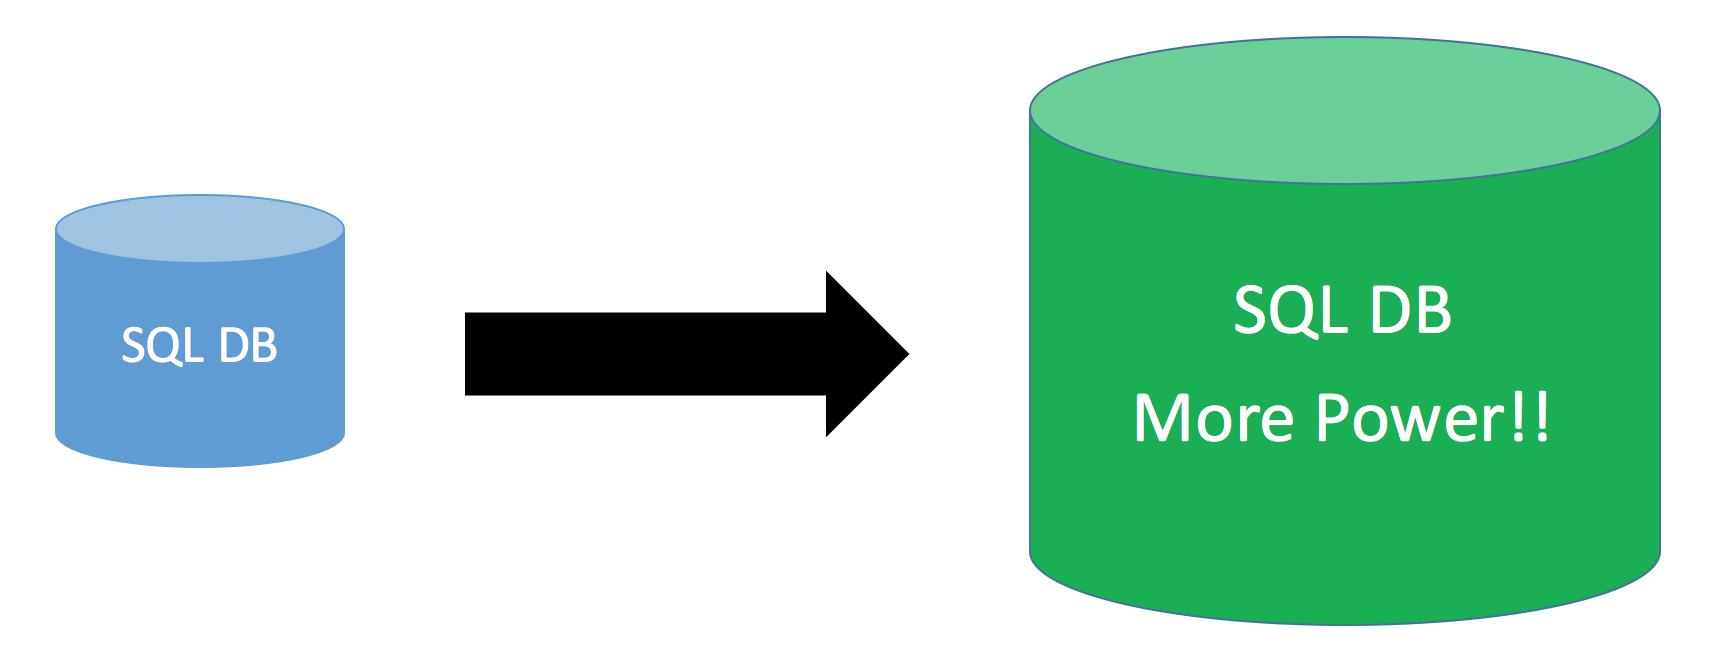
\includegraphics[width=0.7\textwidth]{images/SQL-Scaling-UP}
  \caption{Scaling up a SQL Database}
  \label{fig:Bild1}
\end{figure}

But with exponential growth it is obvious that sooner or later (more sooner than later) you will run into the same problems again. At some point you simply cannot scale up anymore because you already have a monster system, or you cannot afford to buy more expensive hardware.

The next step you could take would be scaling out.

\subsection{Scaling Out}
Scaling out is the opposite of scaling up. Instead of building bigger systems the goal is to distribute the load between many smaller systems.

The simplest way of scaling out an SQL database is using a storage area network (SAN) to store the data. You can then use up to eight SQL servers, attach them to the SAN and let them handle queries. This way load gets distributed between those eight servers.

\begin{figure}[htbp]
  \centering
     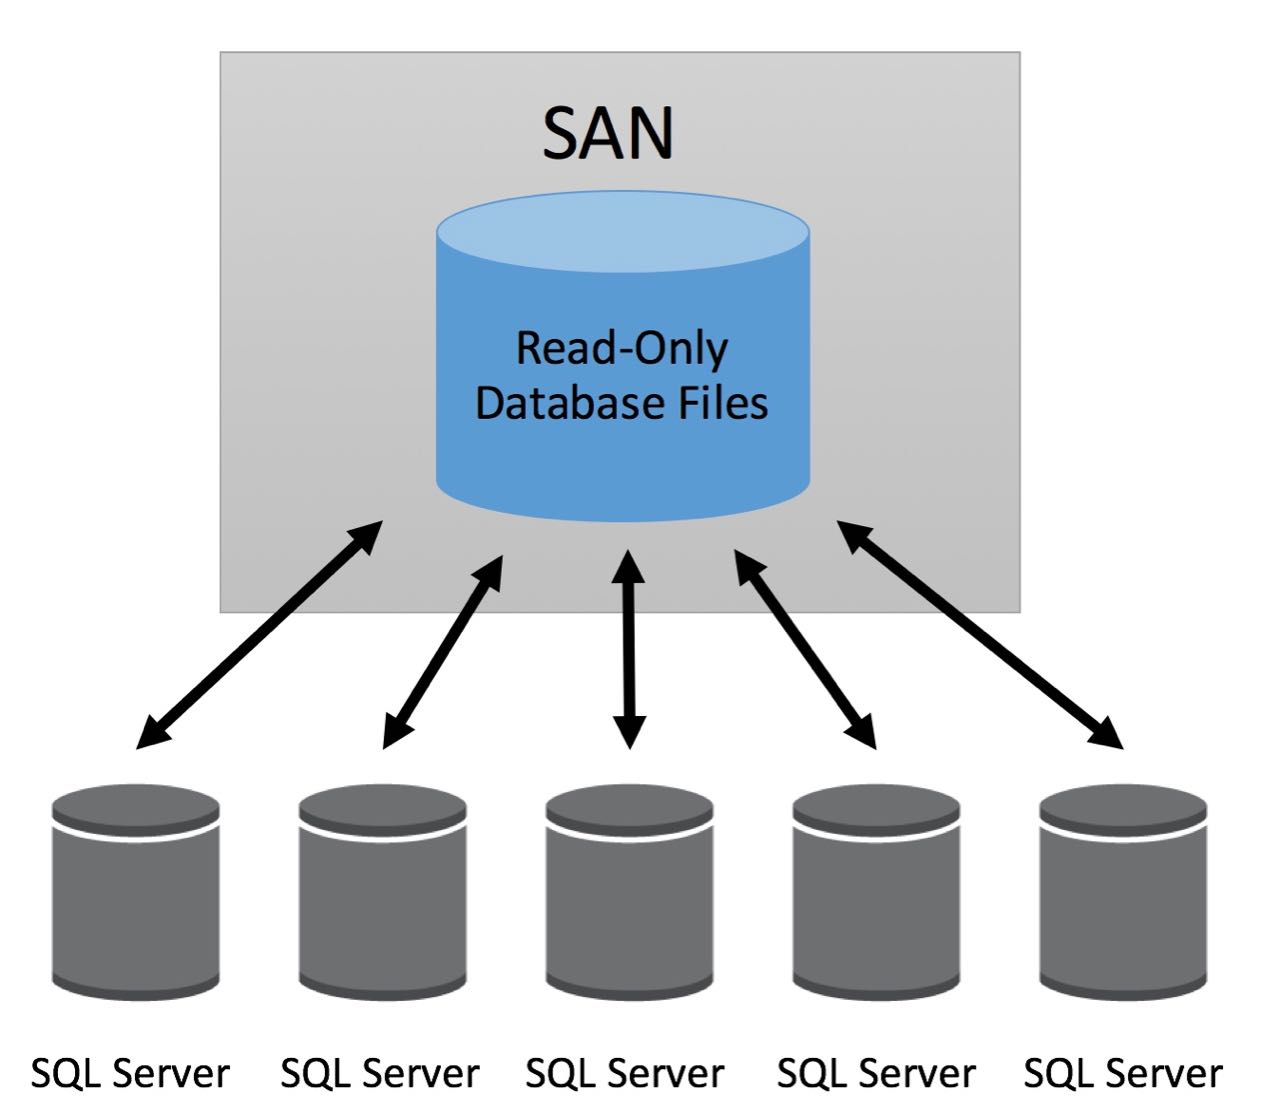
\includegraphics[width=0.7\textwidth]{images/SQL-Scaling-Out}
  \caption{Scaling out a SQL Database}
  \label{fig:Bild1}
\end{figure}

One major downside of this setup is that, because the storage is shared between the sql servers, it can only be used as an read only database. Updates have to be done periodically, for instance once a day. To do updates all SQL servers have to detach from the database. Then, one is attaching the db in read-write mode and refreshing the data. This procedure can take a while if a lot of data needs to be uploaded.

This Link to a Microsoft MSDN page has more options of scaling out an SQL database for you.

I deliberately don’t want to get into details about possible scaling out solutions. The point I am trying to make is that while it is possible to scale out SQL databases it is very complicated.

There is no perfect solution. Every option has its up- and downsides. One common major issue is the administrative effort that you need to take to implement and maintain a scaled out solution.

\subsection{Please Don’t go Big Data}

If you don’t run into scaling issues please, do not use big data tools!

Big data is a expensive thing. A Hadoop cluster for instance needs at least five servers to work properly. More is better.

Believe me this stuff costs a lot of money.

Especially when you are talking the maintenance and development on top big data tools into account.

If you don’t need it it’s making absolutely no sense at all!

On the other side: If you really need big data tools they will save your ass :)



\chapter{Data Warehouse vs Data Lake}

\chapter{Hadoop Platforms | available}
When people talk about big data, one of the first things come to mind is Hadoop. Google’s search for Hadoop returns about 28 million results.

It seems like you need Hadoop to do big data. Today I am going to shed light onto why Hadoop is so trendy.

You will see that Hadoop has evolved from a platform into an ecosystem. It’s design allows a lot of Apache projects and 3rd party tools to benefit from Hadoop.

I will conclude with my opinion on, if you need to learn Hadoop and if Hadoop is the right technology for everybody.

\section{What is Hadoop}

Hadoop is a platform for distributed storing and analyzing of very large data sets.

Hadoop has four main modules: Hadoop common, HDFS, MapReduce and YARN. The way these modules are woven together is what makes Hadoop so successful.

The Hadoop common libraries and functions are working in the background. That’s why I will not go further into them. They are mainly there to support Hadoop’s modules.

\section{What makes Hadoop so popular? | available}
Storing and analyzing data as large as you want is nice. But what makes Hadoop so popular?

Hadoop’s core functionality is the driver of Hadoop’s adoption. Many Apache side projects use it’s core functions.

Because of all those side projects Hadoop has turned more into an ecosystem. An ecosystem for storing and processing big data.

To better visualize this eco system I have drawn you the following graphic. It shows some projects of the Hadoop ecosystem who are closely connected with the Hadoop.

It is not a complete list. There are many more tools that even I don’t know. Maybe I am drawing a complete map in the future.

\begin{figure}[htbp]
  \centering
     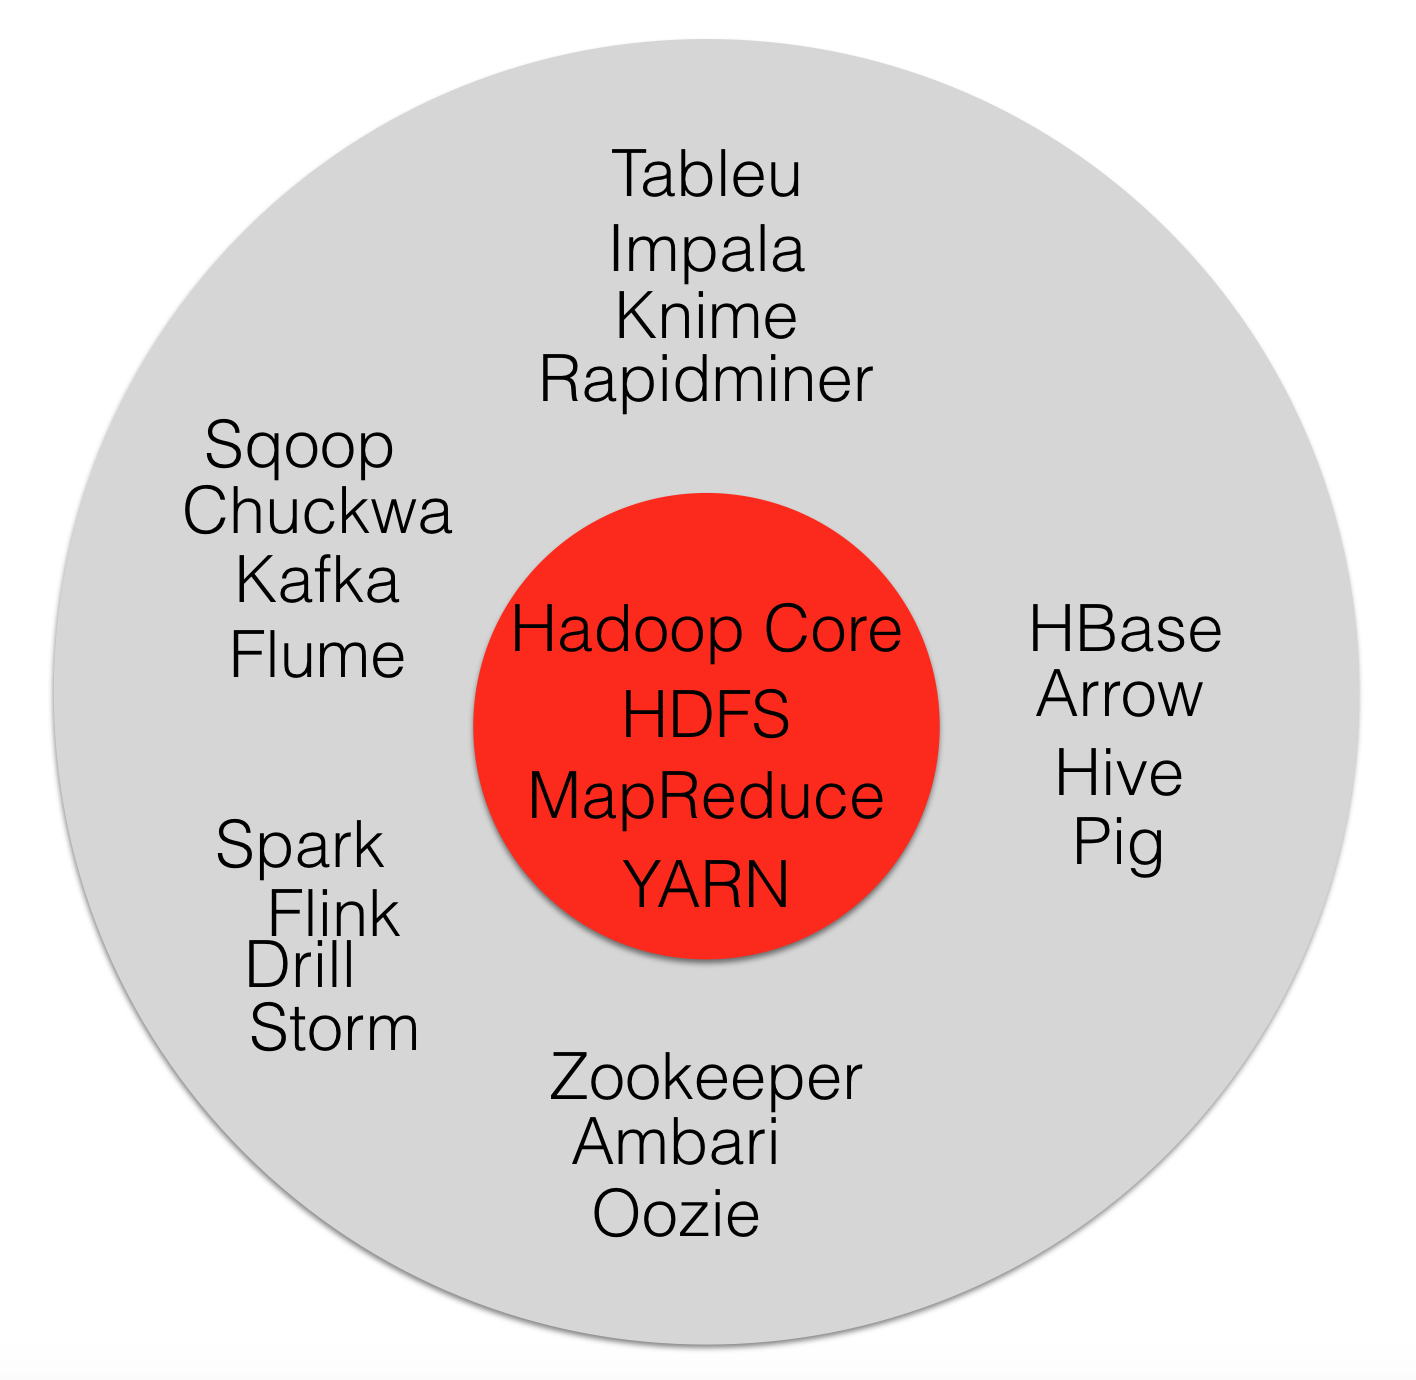
\includegraphics[width=0.9\textwidth]{images/Hadoop-Ecosystem.png}
  \caption{Hadoop Ecosystem Components}
  \label{fig:Bild1}
\end{figure}

\section{Hadoop Ecosystem Components}
Remember my big data platform blueprint? The blueprint has four stages: Ingest, store, analyse and display.

Because of the Hadoop ecosystem” the different tools in these stages can work together perfectly.

Here’s an example:
\begin{figure}[htbp]
  \centering
     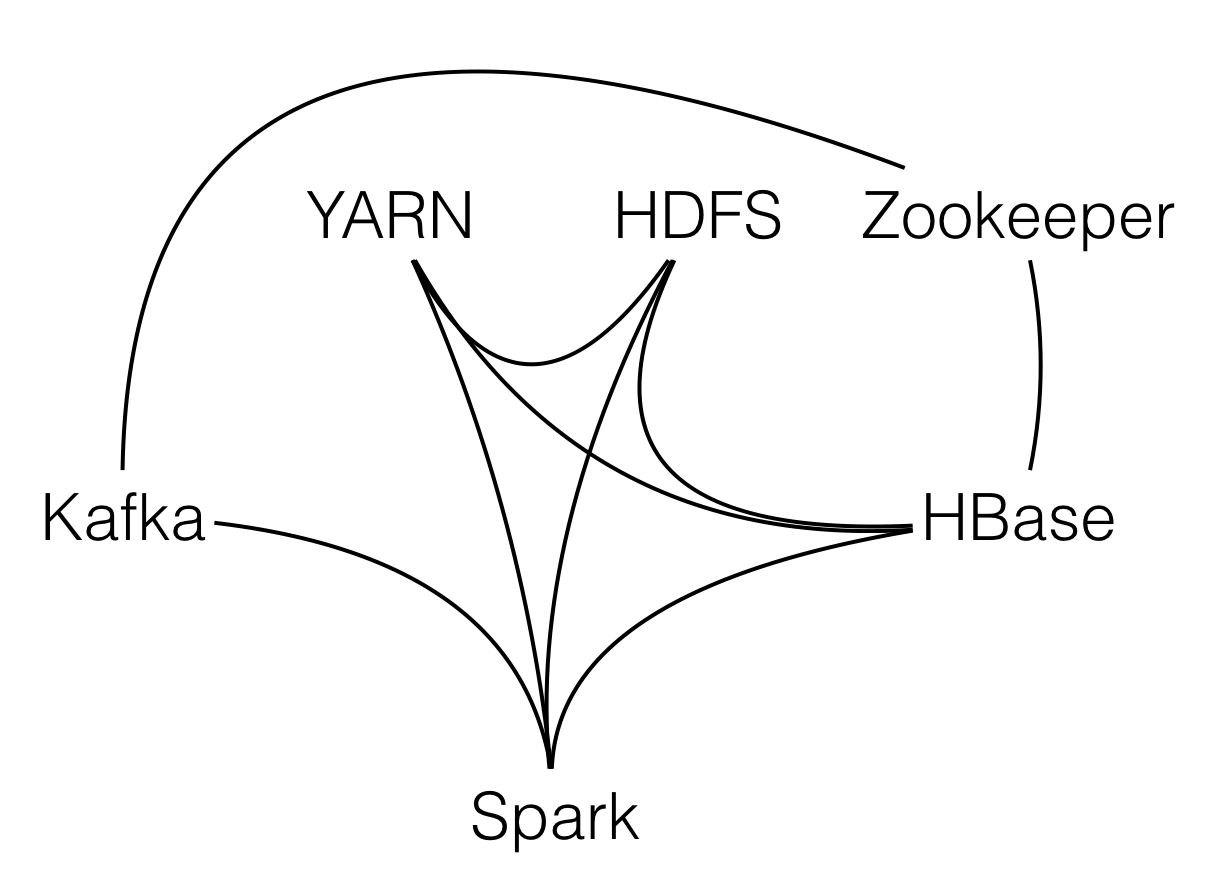
\includegraphics[width=0.9\textwidth]{images/Hadoop-Ecosystem-Connections.png}
  \caption{Connections between tools}
  \label{fig:Bild1}
\end{figure}

You use Apache Kafka to ingest data, and store the it in HDFS. You do the analytics with Apache Spark and as a backend for the display you store data in Apache HBase.

To have a working system you also need YARN for resource management. You also need Zookeeper, a configuration management service to use Kafka and HBase

As you can see in the picture below each project is closely connected to the other.

Spark for instance, can directly access Kafka to consume messages. It is able to access HDFS for storing or processing stored data.

It also can write into HBase to push analytics results to the front end.


The cool thing of such ecosystem is that it is easy to build in new functions.

Want to store data from Kafka directly into HDFS without using Spark?

No problem, there is a project for that. Apache Flume has interfaces for Kafka and HDFS.

It can act as an agent to consume messages from Kafka and store them into HDFS. You even do not have to worry about Flume resource management.

Flume can use Hadoop’s YARN resource manager out of the box.

\begin{figure}[htbp]
  \centering
     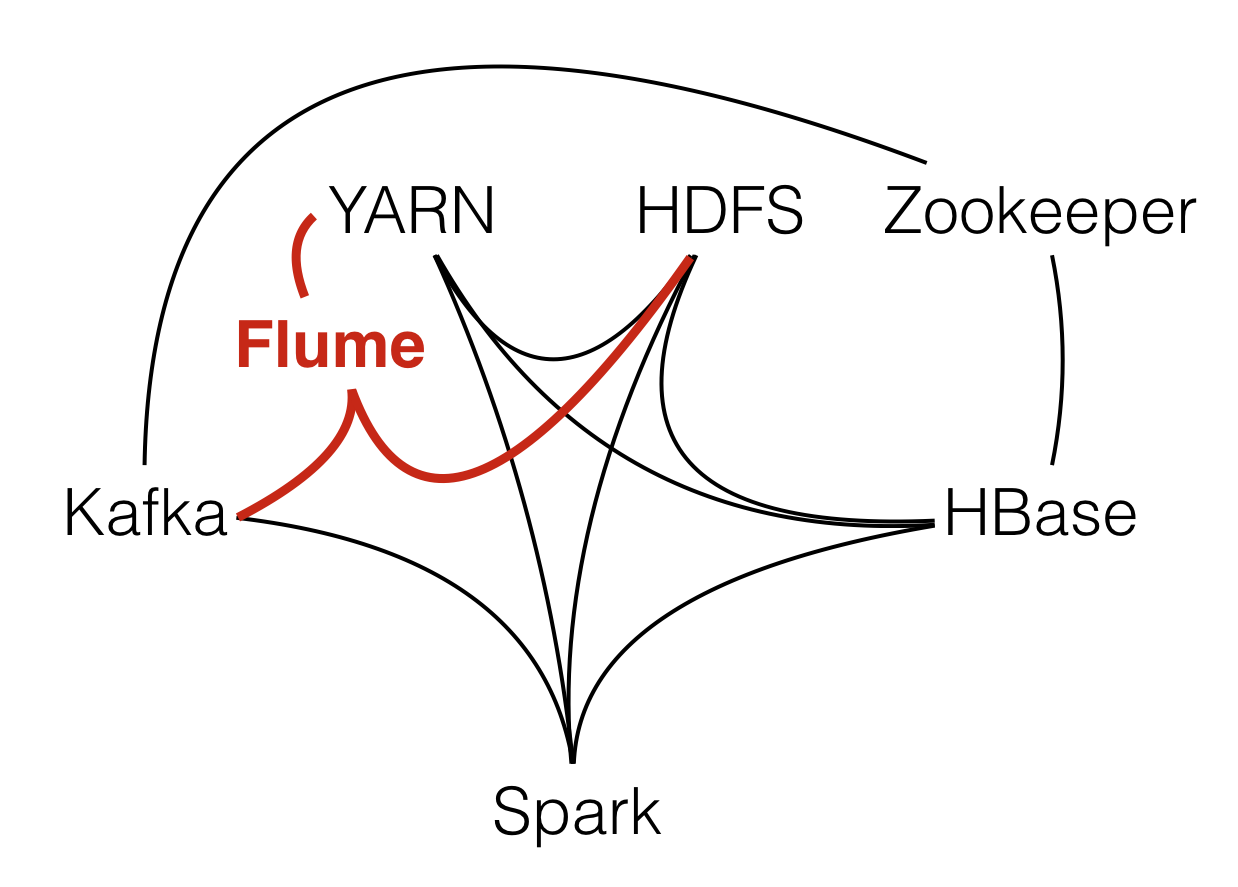
\includegraphics[width=0.9\textwidth]{images/Hadoop-Ecosystem-Connections-Flume.png}
  \caption{Flume Integration}
  \label{fig:Bild1}
\end{figure}



\section{Hadoop Is Everywhere?}

Although Hadoop is so popular it is not the silver bullet. It isn’t the tool that you should use for everything.

Often times it does not make sense to deploy a Hadoop cluster, because it can be overkill. Hadoop does not run on a single server.

You basically need at least five servers, better six to run a small cluster. Because of that. the initial platform costs are quite high.

One option you have is to use a specialized systems like Cassandra, MongoDB or other NoSQL DB’s for storage. Or you move to Amazon and use Amazon’s Simple Storage Service, or S3.

Guess what the tech behind S3 is. Yes, HDFS. That’s why AWS also has the equivalent to MapReduce named Elastic MapReduce.

The great thing about S3 is that you can start very small. When your system grows you don’t have to worry about s3’s server scaling.

\section{Should you learn Hadoop? }

Yes, I definitely recommend you to get to now how Hadoop works and how to use it. As I have shown you in this article, the ecosystem is quite large.

Many big data projects use Hadoop or can interface with it. Thats why it is generally a good idea to know as many big data technologies as possible.

Not in depth, but to the point that you know how they work and how you can use them. Your main goal should be to be able to hit the ground running when you join a big data project.

Plus, most of the technologies are open source. You can try them out for free.
\subsubsection{How does a Hadoop System architecture look like}
\subsubsection{What tools are usually in a with Hadoop Cluster}
Yarn
Zookeeper
HDFS
Oozie
Flume
Hive
\section{How to select Hadoop Cluster Hardware}

\chapter{Is ETL still relevant for Analytics?}
I talked about this in this podcast: https://anchor.fm/andreaskayy/embed/episodes/Is-ETL-Dead-For-Data-Science--Big-Data---PoDS-039-e2b604


\chapter{Docker}

\section{What is docker and what do you use it for | available}
Have you played around with Docker yet? If you’re a data science learner or a data scientist you need to check it out!

It’s awesome because it simplifies the way you can set up development environments for data science. If you want to set up a dev environment you usually have to install a lot of packages and tools.

\subsection{Don’t Mess Up Your System}

What this does is you basically mess up your operating system. If you’re a starter you don’t know which packages you need to install. You don’t know which tools you need to install.

If you want to for instance start with Jupyter notebooks you need to install that on your PC somehow. Or you need to start installing tools like PyCharmor Anaconda.

All that gets added to your system and so you mess up your system more and more and more. What Docker brings you, especially if you’re on a Mac or a Linux system is simplicity.

\subsection{Preconfigured Images}

Because it is so easy to install on those systems. Another cool thing about docker images is you can just search them in the Docker store, download them and install them on your system.

Running them in a completely pre-configured environment. You don’t need to think about stuff you go to the Docker library you search for deep learning GPU and Python.

You get a list of images you can download. You download one, start it up, you go to the browser hit up the URL and just start coding.

Start doing the work. The only other thing you need to do is bind some drives to that instance so you can exchange files. And then that’s it!

There is no way that you can crash or mess up your system. It’s all encapsulated into Docker.Why this works is because Docker has natively access to your hardware.

\subsection{Take It With You}

It’s not a completely virtualized environment like a VirtualBox. An image has the upside that you can take it wherever you want. So if your on your PC at home use that there.

Make a quick build, take the image and go somewhere else. Install the image which is usually quite fast and just use it like you’re at home.

It’s that awesome!

\section{Kubernetes Container Deployment}

I am getting into Docker a lot more myself. For a bit different reasons.

What I’m looking for is using Docker with Kubernetes. With Kubernetes you can automate the whole container deployment process.

The idea with is that you have a cluster of machines. Lets say you have 10 server cluster and you run Kubernetes on them.

Kubernetes lets you spin up Docker containers on-demand to execute tasks. You can set up how much resources like CPU, RAM, Network, Docker container can use.

You can basically spin up containers, on the cluster on demand. When ever you need to do a analytics task.

Perfect for Data Science.
\section{How to create, start,stop a Container}
\section{Docker micro services?}
\section{Kubernetes}
\section{Why and how to do Docker container orchestration}
Podcast about how data science learners use Docker (for data scientists): https://anchor.fm/andreaskayy/embed/episodes/Learn-Data-Science-Go-Docker-e10n7u





\chapter{REST APIs}
APIs, Application Programming Interfaces are the cornerstones of any great data platform. 

\begin{table}[h]
\begin{tabular}{ll}
\hline
\multicolumn{2}{l}{\textbf{Podcast Episode:} \#033 How APIs Rule The World} \\ \hline
\multicolumn{2}{p{15cm}}{Strong APIs make a good platform. In this episode I talk about why you need APIs and why Twitter is a great example. Especially JSON APIs are my personal favorite. Because JSON is also important in the Big Data world, for instance in log analytics. How? Check out this episode!}         \\ \hline
\multicolumn{1}{l|}{Audio}     & \href{https://anchor.fm/andreaskayy/episodes/How-APIs-Rule-The-World--PoDS-033-e24ttq}{Click here to listen}   \\ \hline
\end{tabular}
\end{table}

\section{HTTP Post/Get}
\section{API Design}
In this podcast episode we look into the Twitter API. It's a great example how to build an API

\begin{table}[h]
\begin{tabular}{ll}
\hline
\multicolumn{2}{l}{\textbf{Podcast Episode:} \#081 Twitter API Research Data Engineering Course Part 5} \\ \hline
\multicolumn{2}{p{15cm}}{In this episode we look into the Twitter API documentation, which I love by the way. How can we get old tweets for a certain hashtags and how to get current live tweets for these hashtags?}         \\ \hline
\multicolumn{1}{l|}{Audio}     & \href{https://anchor.fm/andreaskayy/episodes/081-How-to-get-tweets-from-the-Twitter-API-e45j32}{Click here to listen}   \\
\multicolumn{1}{l|}{Youtube}   & \href{https://youtu.be/UnAXKxeIlyg}{Click here to watch}   \\ \hline
\end{tabular}
\end{table}


\section{Implementation}
\section{OAuth security}

\chapter{Databases}

\section{SQL Databases}

\subsection{Database Design}
\subsection{SQL Queries}
\subsection{Stored Procedures}
\subsection{ODBC/JDBC Server Connections}

\section{NoSQL Stores}
\subsection{KeyValue Stores (HBase)}
\subsection{Document Store HDFS | available}

The Hadoop distributed file system, or HDFS, allows you to store files in Hadoop. The difference between HDFS and other file systems like NTFS or EXT is that it is a distributed one.

What does that mean exactly?

A typical file system stores your data on the actual hard drive. It is hardware dependent.

If you have two disks then you need to format every disk with its own file system. They are completely separate.

You then decide on which disk you physically store your data.

HDFS works different to a typical file system. HDFS is hardware independent.

Not only does it span over many disks in a server. It also spans over many servers.

HDFS will automatically place your files somewhere in the Hadoop server collective.

It will not only store your file, Hadoop will also replicate it two or three times (you can define that). Replication means replicas of the file will be distributed to different servers.

\begin{figure}[htbp]
  \centering
     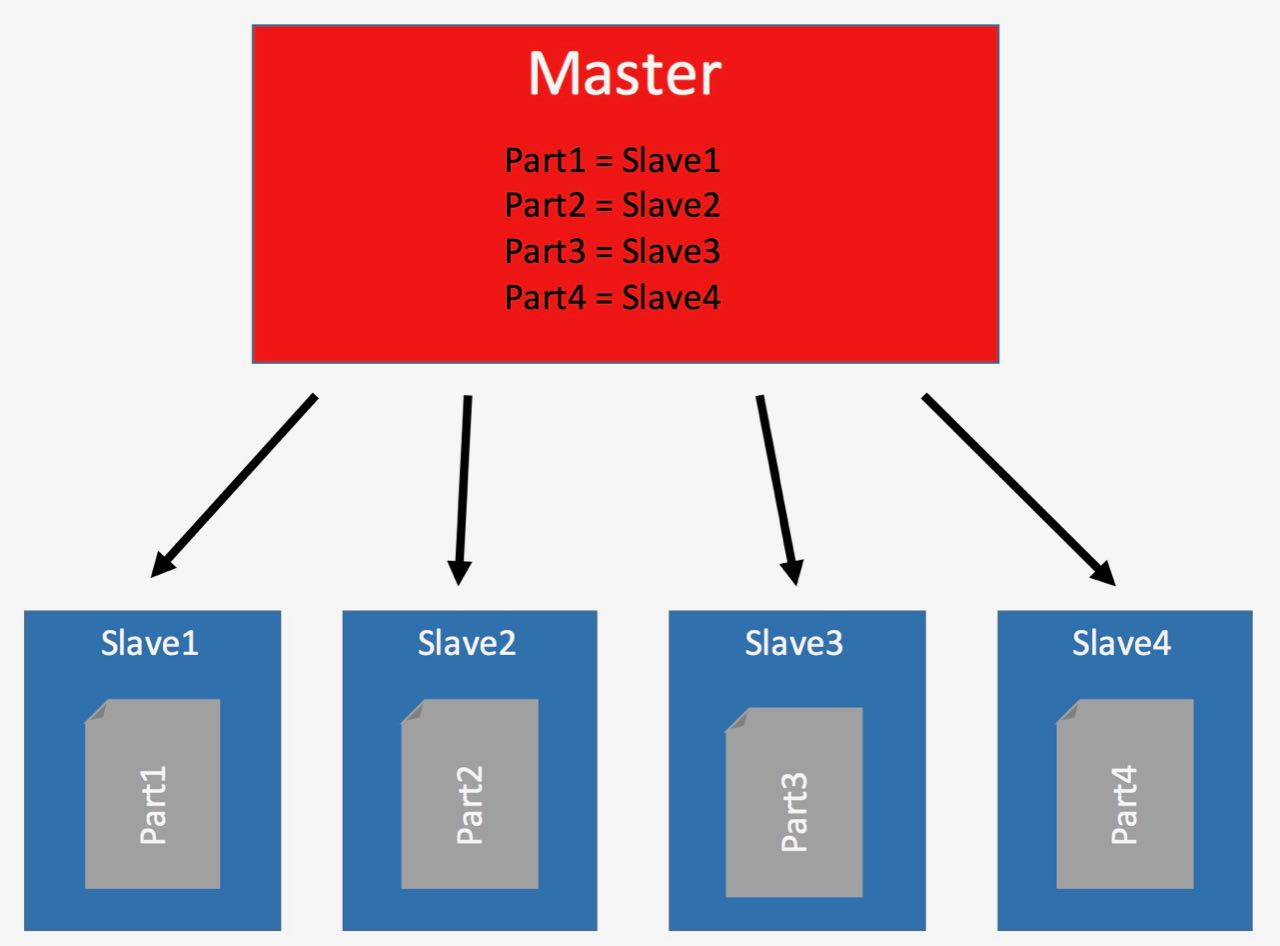
\includegraphics[width=0.9\textwidth]{images/HDFS-Master-DataNodes}
  \caption{HDFS Master and Data Nodes}
  \label{fig:Bild1}
\end{figure}

This gives you superior fault tolerance. If one server goes down, then your data stays available on a different server.

Another great thing about HDFS is, that there is no limit how big the files can be. You can have server log files that are terabytes big.

How can files get so big? HDFS allows you to append data to files. Therefore, you can continuously dump data into a single file without worries.

HDFS physically stores files different then a normal file system. It splits the file into blocks.

These blocks are then distributed and replicated on the Hadoop cluster. The splitting happens automatically.

\begin{figure}[htbp]
  \centering
     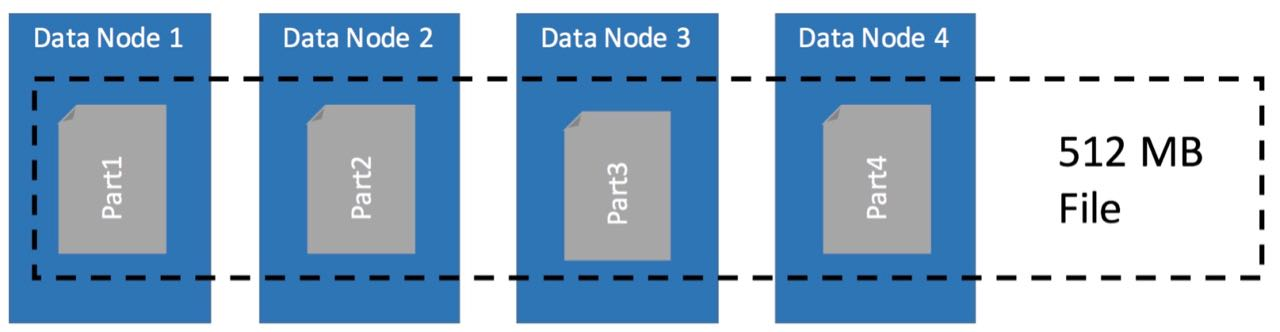
\includegraphics[width=0.9\textwidth]{images/HDFS-Distributed-FileSystem}
  \caption{Distribution of Blocks for a 512MB File}
  \label{fig:Bild1}
\end{figure}

In the configuration you can define how big the blocks should be. 128 megabyte or 1 gigabyte?

No problem at all.

This mechanic of splitting a large file in blocks and distributing them over the servers is great for processing.
See the MapReduce section for an example.

\subsection{Document Store MongoDB}
\subsection{Hive Warehouse}
\subsection{Impala}
\subsection{Kudu}

\subsection{Time Series Databases}
DalmatinerDB
InfluxDB
Prometheus
Riak TS
OpenTSDB
KairosDB
Elasticsearch
Druid
\subsection{MPP Databases (Greenplum)}


\chapter{Data Processing / Analytics - Frameworks}
\section{MapReduce}

Since the early days of the Hadoop eco system, the MapReduce framework is one of the main components of Hadoop alongside the Hadoop file system HDFS.

Google for instance used MapReduce to analyse stored html content of websites through counting all the html tags and all the words and combinations of them (for instance headlines). The output was then used to create the page ranking for Google Search.

That was when everybody started to optimise his website for the google search. Serious search engine optimisation was borne. That was the year 2004.

How MapReduce is working is, that it processes data in two phases: The map phase and the reduce phase.

In the map phase, the framework is reading data from HDFS. Each dataset is called an input record.

Then there is the reduce phase. In the reduce phase, the actual computation is done and the results are stored. The storage target can either be a database or back HDFS or something else.

After all it’s Java – so you can implement what you like.

The magic of MapReduce is how the map and reduce phase are implemented and how both phases are working together.

The map and reduce phases are parallelised. What that means is, that you have multiple map phases (mappers) and reduce phases (reducers) that can run in parallel on your cluster machines.

Here's an example how such a map and reduce process works with data:

\begin{figure}[htbp]
  \centering
     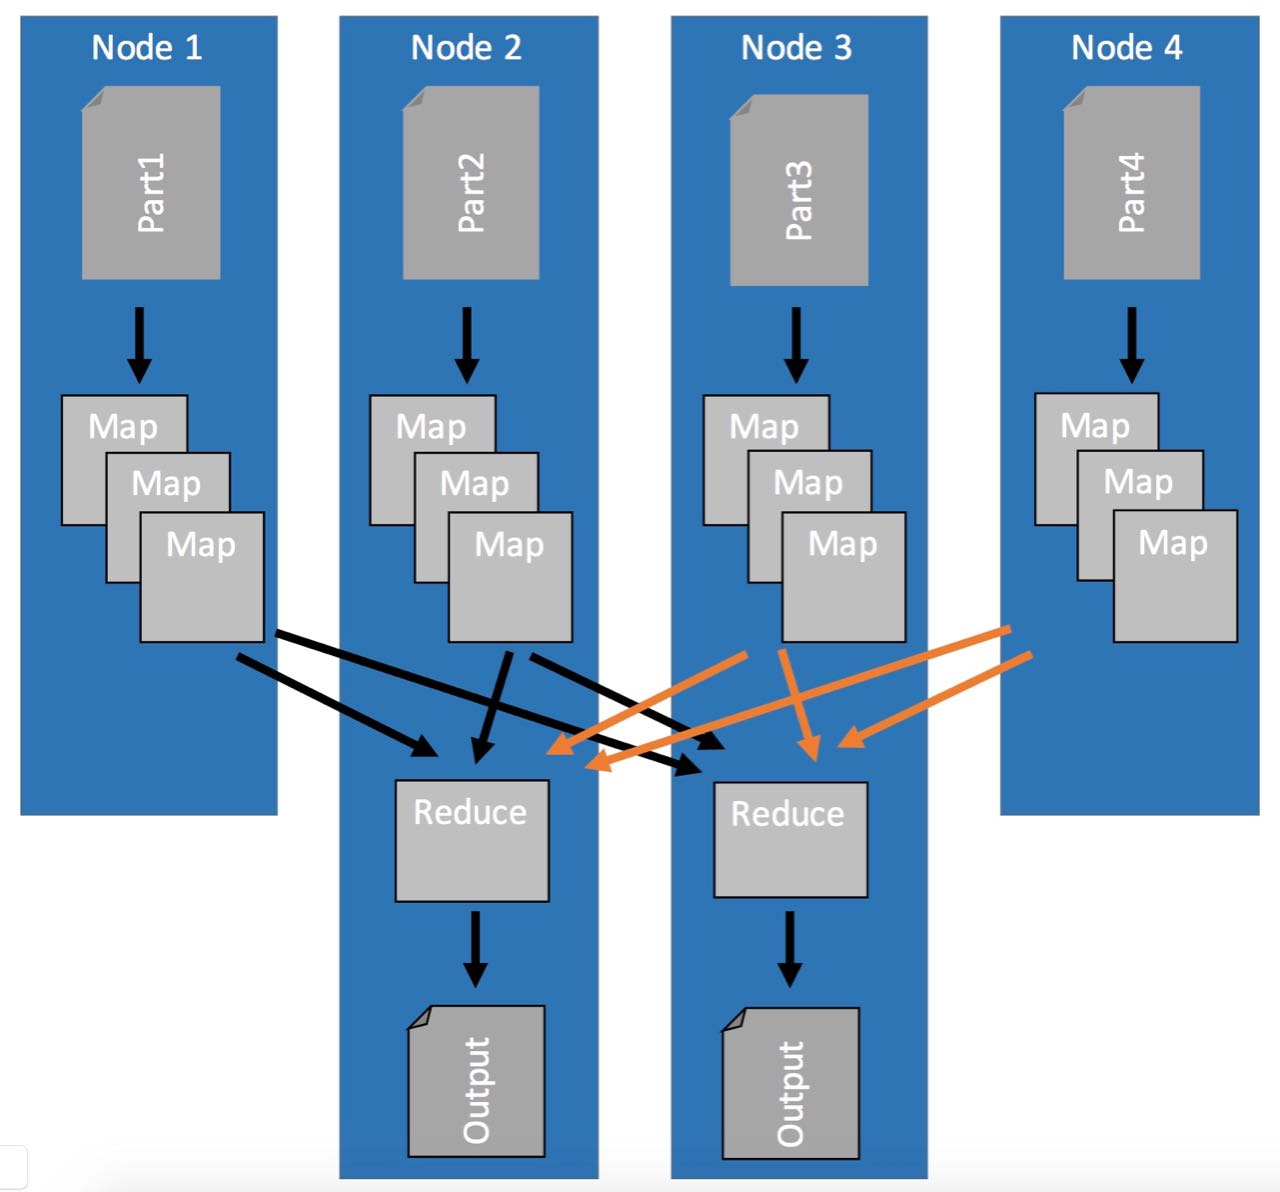
\includegraphics[width=0.9\textwidth]{images/MapReduce-Process-Detailed}
  \caption{Mapping of input files and reducing of mapped records}
  \label{fig:Bild1}
\end{figure}

\subsection{How does MapReduce work -- available}

First of all, the whole map and reduce process relies heavily on using key/value pairs. That’s what the mappers are for.

In the map phase input data, for instance a file, gets loaded and transformed into key/value pairs.

When each map phase is done it sends the created key/value pairs to the reducers where they are getting sorted by key. This means, that an input record for the reduce phase is a list of values from the mappers that all have the same key.

Then the reduce phase is doing the computation of that key and its values and outputting the results.

How many mappers and reducers can you use in parallel? The number of parallel map and reduce processes depends on how many CPU cores you have in your cluster. Every mapper and every reducer is using one core.

This means that the more CPU cores you actually have, the more mappers you can use, the faster the extraction process can be done. The more reducers you are using the faster the actual computation is being done.

To make this more clear, I have prepared an example:

\subsection{Example}
As I said before, MapReduce works in two stages, map and reduce. Often these stages are explained with a word count task.

Personally, I hate this example because counting stuff is to trivial and does not really show you what you can do with MapReduce. Therefore, we are going to use a more real world use-case from the world of the internet of things (IoT).

IoT applications create an enormous amount of data that has to be processed. This data is generated by physical sensors who take measurements, like room temperature at 8.00 o’Clock.

Every measurement consists of a key (the timestamp when the measurement has been taken) and a value (the actual value measured by the sensor).

Because you usually have more than one sensor on your machine, or connected to your system, the key has to be a compound key. Compound keys contain additionally to the measurement time information about the source of the signal.

But, let’s forget about compound keys for now. Today we have only one sensor. Each measurement outputs key/value pairs like: Timestamp-Value.

The goal of this exercise is to create average daily values of that sensor’s data.

The image below shows how the map and reduce process works.

First, the map stage loads unsorted data (input records) from the source (e.g. HDFS) by key and value (key:2016-05-01 01:02:03, value:1).

Then, because the goal is to get daily averages, the hour:minute:second information is cut from the timestamp.

That is all that happens in the map phase, nothing more.

After all parallel map phases are done, each key/value pair gets sent to the one reducer who is handling all the values for this particular key.

Every reducer input record then has a list of values and you can calculate (1+5+9)/3, (2+6+7)/3 and (3+4+8)/3. That’s all.

\begin{figure}[htbp]
  \centering
     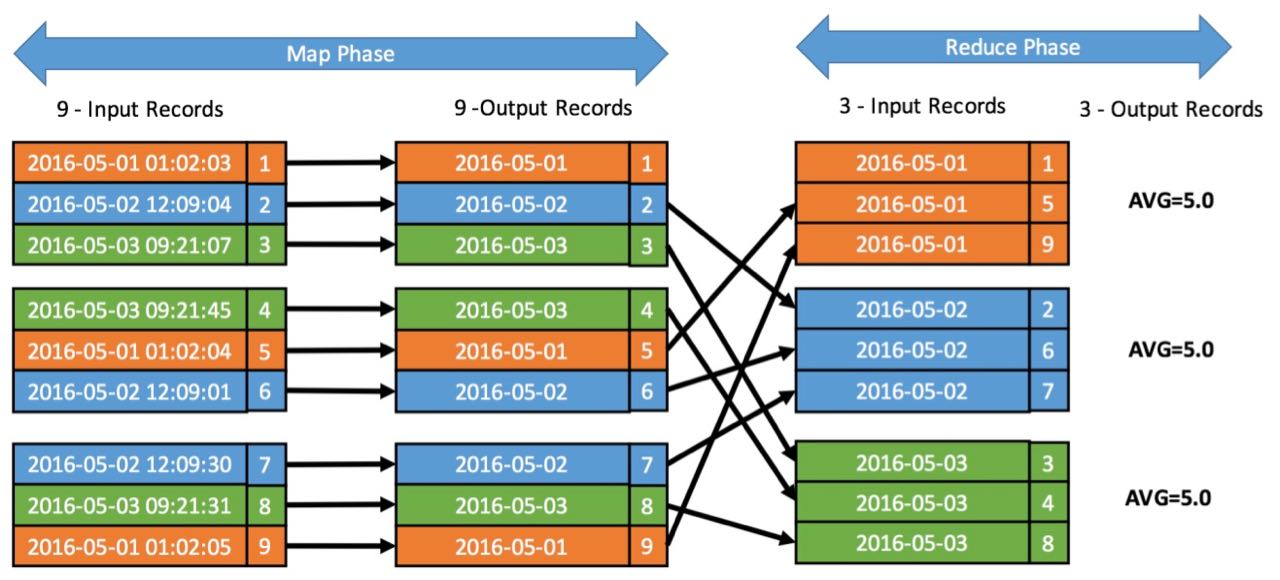
\includegraphics[width=0.9\textwidth]{images/MapReduce-Time-Series-example}
  \caption{MapReduce Example of Time Series Data}
  \label{fig:Bild1}
\end{figure}

What do you think you need to do to generate minute averages?

Yes, you need to cut the key differently. You then would need to cut it like this: “2016-05-01 01:02”. Keeping the Hour and minute information in the key.

What you can also see is, why map reduce is so great for doing parallel work. In this case, the map stage could be done by nine mappers in parallel because each map is independent from all the others.

The reduce stage could still be done by three tasks in parallel. One each for orange, blue and one for green.

That means, if your dataset would be 10 times as big and you’d have 10 times the machines, the time to do the calculation would be the same.

\subsection{What is the limitation of MapReduce? -- available}
MapReduce is awesome for simpler analytics tasks, like counting stuff. It just has one flaw: It has only two stages Map and Reduce.

\begin{figure}[htbp]
  \centering
     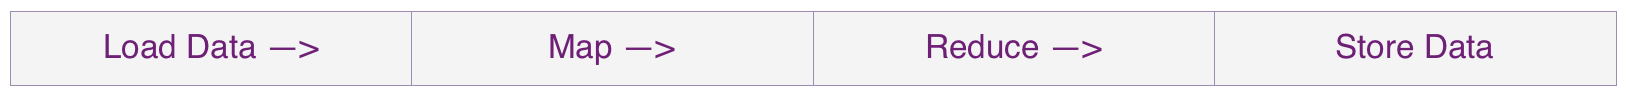
\includegraphics[width=0.9\textwidth]{images/MapReduce-Process}
  \caption{The Map Reduce Process}
  \label{fig:Bild1}
\end{figure}

First MapReduce loads the data from HDFS into the mapping function. There you prepare the input data for the processing in the reducer. After the reduce is finished the results get written to the data store.

The problem with MapReduce is that there is no simple way to chain multiple map and reduce processes together. At the end of each reduce process the data must be stored somewhere.

This fact makes it very hard to do complicated analytics processes. You would need to chain MapReduce jobs together.

Chaining jobs with storing and loading intermediate results just makes no sense.

Another issue with MapReduce is that it is not capable of streaming analytics. Jobs take some time to spin up, do the analytics and shut down. Basically Minutes of wait time are totally normal.

This is a big negative point in a more and more real time data processing world.



\section{Apache Spark}
I talked about the three methods of data streaming in this podcast: https://anchor.fm/andreaskayy/embed/episodes/Three-Methods-of-Streaming-Data-e15r6o


\subsection{What is the difference to MapReduce? -- available}
Spark is a complete in memory framework. Data gets loaded from, for instance hdfs, into the memory of workers.

There is no longer a fixed map and reduce stage. Your code can be as complex as you want.

Once in memory, the input data and the intermediate results stay in memory (until the job finishes). They do not get written to a drive like with MapReduce.

This makes Spark the optimal choice for doing complex analytics. It allows you for instance to do Iterative processes. Modifying a dataset multiple times in order to create an output is totally easy.

Streaming analytics capability is also what makes spark so great. Spark has natively the option to schedule a job to run every X seconds or X milliseconds.

As a result, Spark can deliver you results from streaming data in “real time”.


\subsection{How does Spark fit to Hadoop? -- available}
There are some very misleading articles out there titled Spark or Hadoop, Spark is better than Hadoop or even Spark is replacing Hadoop.

\begin{figure}[htbp]
  \centering
     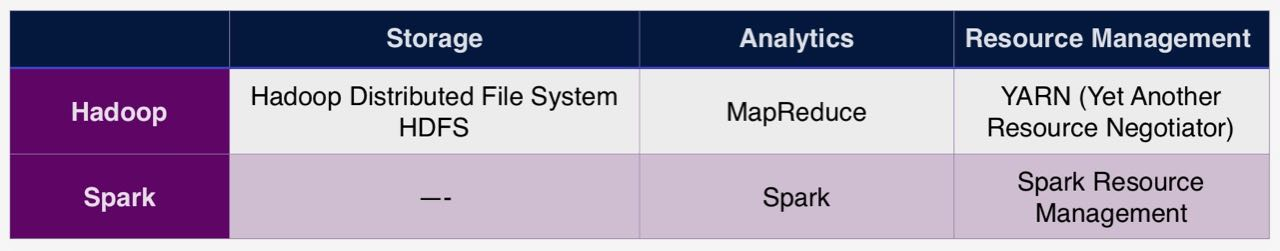
\includegraphics[width=0.9\textwidth]{images/Table-Hadoop-and-Spark}
  \caption{Hadoop vs Spark capabilities}
  \label{fig:Bild1}
\end{figure}



So, it's time to show you the differences between Spark and Hadoop. After this you will know when and for what you should use Spark and Hadoop.

You’ll also understand why Hadoop or Spark is the totally wrong question.

\subsection{Where's the difference?}
To make it clear how Hadoop differs from Spark I created this simple feature table:


Hadoop is used to store data in the Hadoop Distributed File System (HDFS). It can analyse the stored data with MapReduce and manage resources with YARN.

However, Hadoop is more than just storage, analytics and resource management. There’s a whole eco system of tools around the Hadoop core. I’ve written about tis eco system in this article: What is Hadoop and why is it so freakishly popular. You should check it out as well.

Compared to Hadoop, Spark is “just” an analytics framework. It has no storage capability. Although it has a standalone resource management, you usually don’t use that feature.

\subsection{Spark and Hadoop is a perfect fit}
So, if Hadoop and Spark are not the same things, can they work together?

Absolutely! Here’s how the first picture will look if you combine Hadoop with Spark:


As Storage you use the Hadoop distributed file system. Analytics is done with Apache Spark and Yarn is taking care of the resource management.

Why does that work so well together?

From a platform architecture perspective, Hadoop and Spark are usually managed on the same cluster. This means on each server where a HDFS data node is running, a spark worker thread runs as well.

In distributed processing, network transfer between machines is a large bottle neck. Transferring data within a machine reduces this traffic significantly.

Spark is able to determine on which data node the needed data is stored. This allows a direct load of the data from the local storage into the memory of the machine.

This reduces network traffic a lot.

\subsection{Spark on YARN:} You need to make sure that your physical resources are distributed perfectly between the services. This is especially the case when you run Spark workers with other Hadoop services on the same machine.

It just would not make sense to have two resource managers managing the same server’s resources. Sooner or later they will get in each others way.

That’s why the Spark standalone resource manager is seldom used.

So, the question is not Spark or Hadoop. The question has to be: Should you use Spark or MapReduce alongside Hadoop’s HDFS and YARN.

\subsection{My simple rule of thumb:}

If you are doing simple batch jobs like counting values or doing calculating averages: Go with MapReduce.

If you need more complex analytics like machine learning or fast stream processing: Go with Apache Spark.

\subsection{Available Languages -- available}

Spark jobs can be programmed in a variety of languages. That makes creating analytic processes very user-friendly for data scientists.

Spark supports Python, Scala and Java. With the help of SparkR you can even connect your R program to a Spark cluster.

If you are a data scientist who is very familiar with Python just use Python, its great. If you know how to code Java I suggest you start using Scala.

Spark jobs are easier to code in Scala than in Java. In Scala you can use anonymous functions to do processing.

This results in less overhead, it is a much cleaner, simpler code.

With Java 8 simplified function calls were introduced with lambda expressions. Still, a lot of people, including me prefer Scala over Java.

\subsection{How to do stream processing}
\subsection{How to do batch processing}
\subsection{How does Spark use data from Hadoop -- available}
Another thing is data locality. I always make the point, that processing data locally where it is stored is the most efficient thing to do.

That’s exactly what Spark is doing. You can and should run Spark workers directly on the data nodes of your Hadoop cluster.

Spark can then natively identify on what data node the needed data is stored. This enables Spark to use the worker running on the machine where the data is stored to load the data into the memory.

\begin{figure}[htbp]
  \centering
     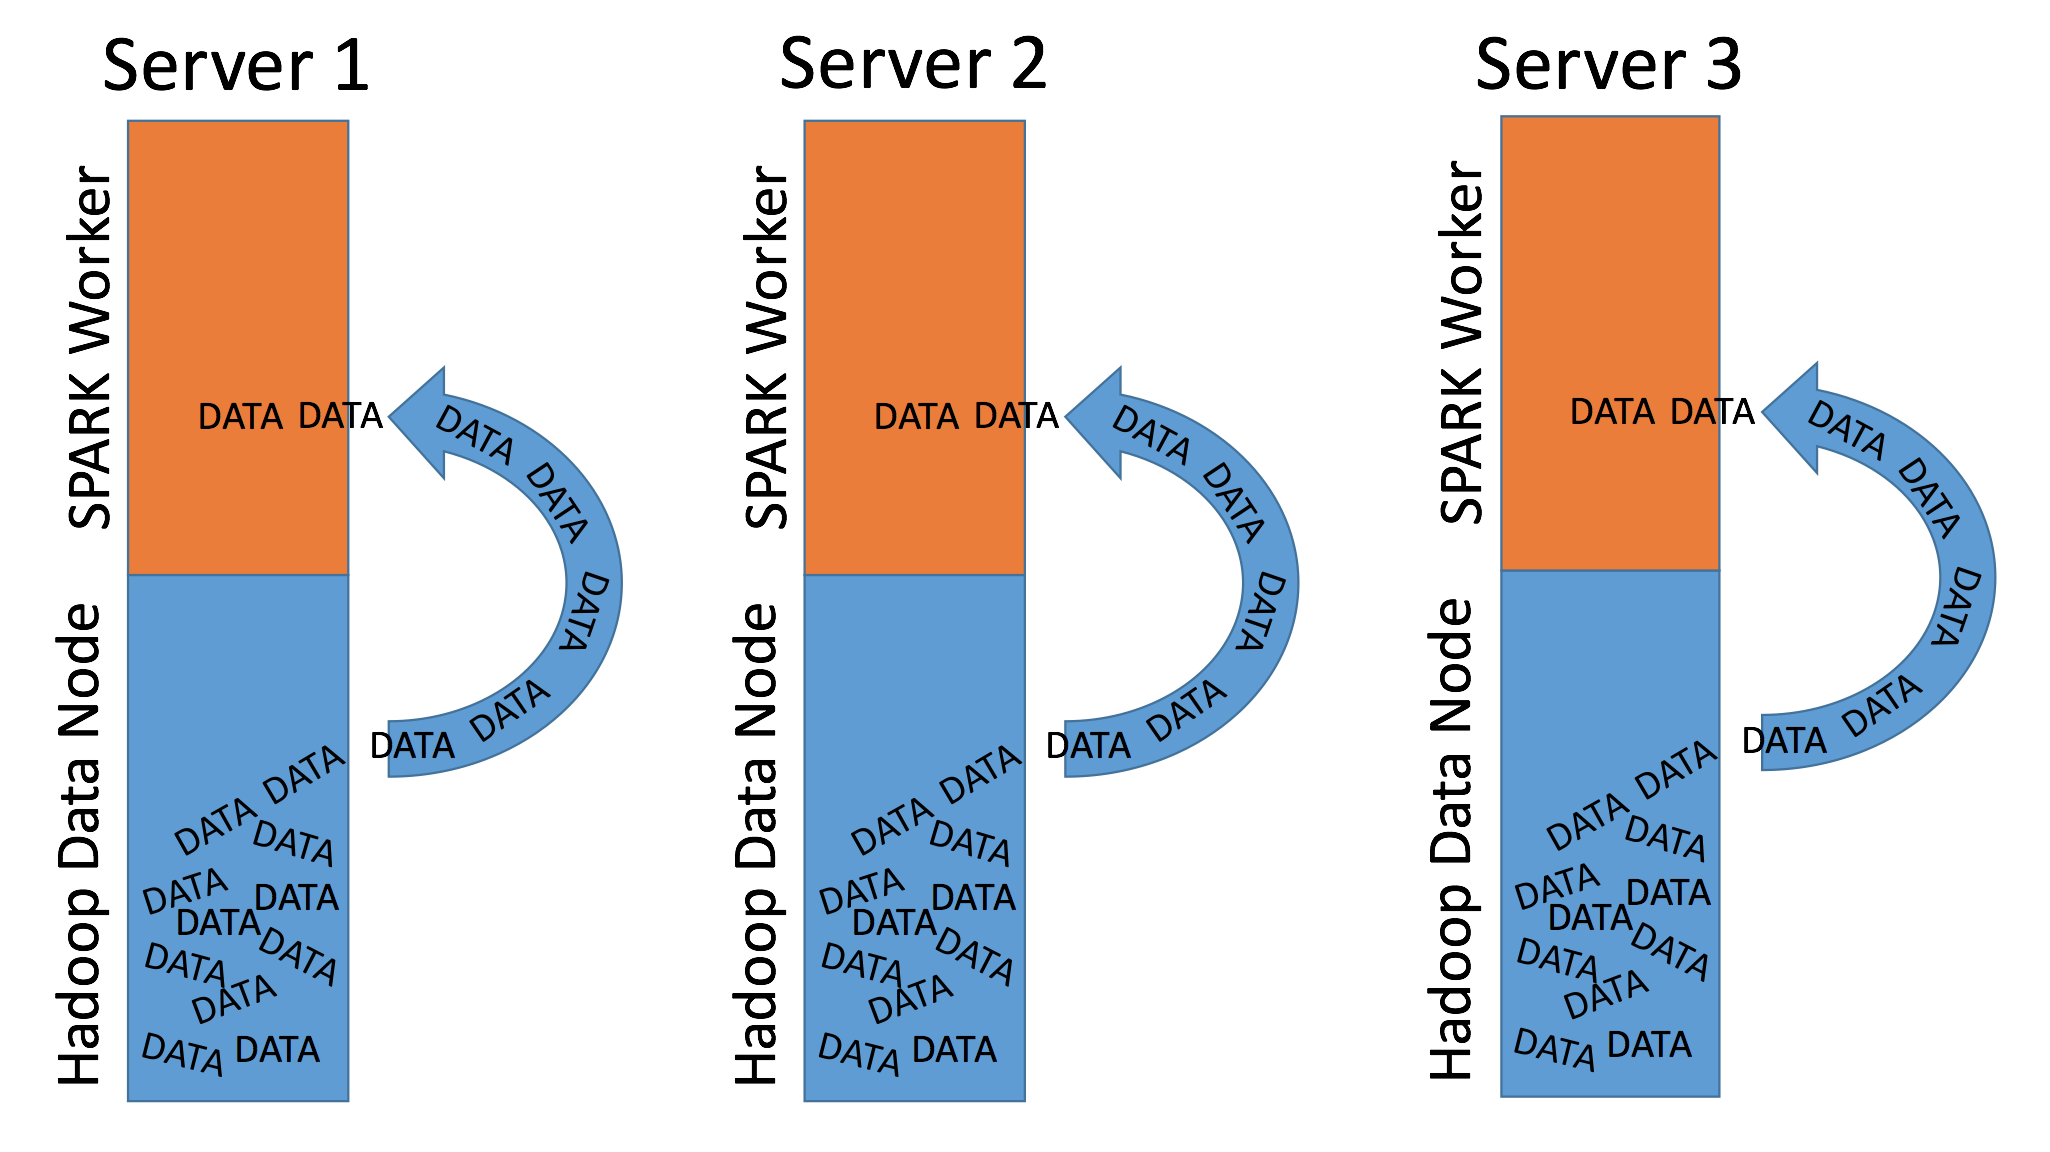
\includegraphics[width=0.9\textwidth]{images/Spark-Data-Locality}
  \caption{Spark Using Hadoop Data Locality}
  \label{fig:Bild1}
\end{figure}

The downside of this setup is that you need more expensive servers. Because Spark processing needs stronger servers with more RAM and CPUs than a “pure” Hadoop setup.


\section{What is a RDD and what is a DataFrame?}
\section{Spark coding with Scala}
\section{Spark coding with Python}
\section{How and why to use SparkSQL?}
\section{Machine Learning on Spark? (Tensor Flow)}

\section{MLlib:} The machine learning library MLlib is included in Spark so there is often no need to import another library.

I have to admit because I am not a data scientist I am not an expert in machine learning.

From what I have seen and read though the machine learning framework MLlib is a nice treat for data scientists wanting to train and apply models with Spark.

\section{Spark Setup -- available}
From a solution architect’s point of view Spark is a perfect fit for Hadoop big data platforms. This has a lot to do with cluster deployment and management.

Companies like Cloudera, MapR or Hortonworks include Spark into their Hadoop distributions. Because of that, Spark can be deployed and managed with the clusters Hadoop management web fronted.

This makes the process for deploying and configuring a Spark cluster very quick and admin friendly.

\section{Spark Resource Management -- available}
When running a computing framework you need resources to do computation: CPU time, RAM, I/O and so on. Out of the box Spark can manage resources with it’s stand-alone resource manager.

If Spark is running in an Hadoop environment you don’t have to use Spark’s own stand-alone resource manager. You can configure Spark to use Hadoop’s YARN resource management.

Why would you do that?
It allows YARN to efficiently allocate resources to your Hadoop and Spark processes.

Having a single resource manager instead of two independent ones makes it a lot easier to configure the resource management.

\begin{figure}[htbp]
  \centering
     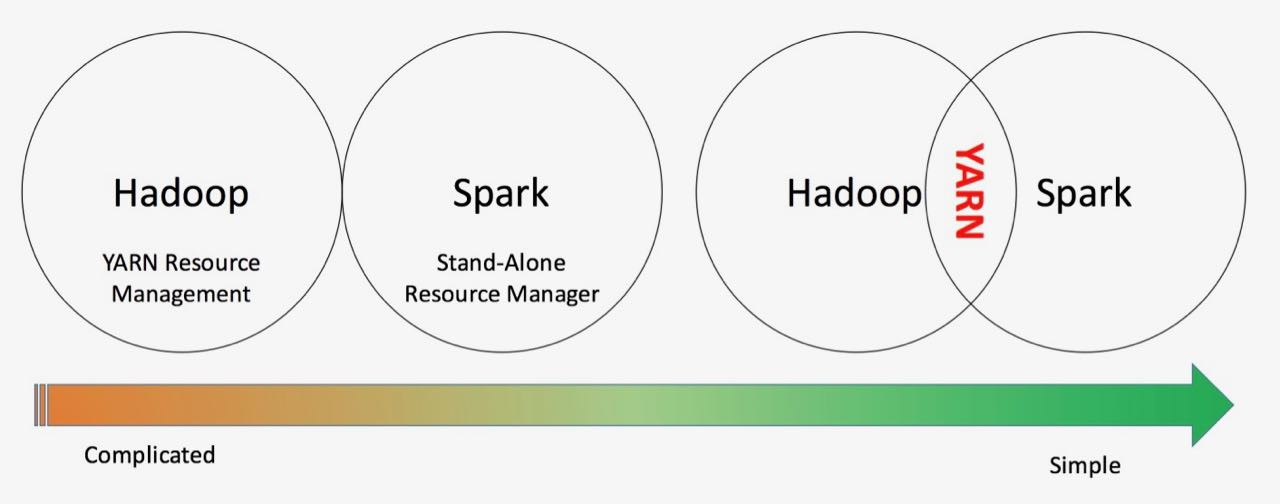
\includegraphics[width=0.9\textwidth]{images/Spark-Yarn}
  \caption{Spark Resource Management With YARN}
  \label{fig:Bild1}
\end{figure}


\chapter{Apache Kafka}

\section{Why a message queue tool?}
\section{Kakfa architecture}
\section{What are topics}
\section{What does Zookeeper have to do with Kafka}
\section{How to produce and consume messages}

My YouTube video how to set up Kafka at home: https://youtu.be/7F9tBwTUSeY

My YouTube video how to write to Kafka: https://youtu.be/RboQBZvZCh0

\chapter{Machine Learning}
My podcast about how to do machine learning in production: https://anchor.fm/andreaskayy/embed/episodes/Machine-Learning-In-Production-e11bbk

\section{Training and Applying models}
\section{What is deep learning}
\section{How to do Machine Learning in production | available}
Machine learning in production is using stream and batch processing. In the batch processing layer you are creating the models, because you have all the data available for training.

In the stream in processing layer you are using the created models, you are applying them to new data.

The idea that you need to incorporate is this is a constant a constant cycle. Training, applying, re-training, pushing into production and applying.

What you don’t want to do is, you don’t want to do this manually. You need to figure out a process of automatic retraining and automatic pushing to into production of models.

In the retraining phase the system automatically evaluates the training. If the model no longer fits it works as long as it needs to create a good model.

After the evaluation of the model is complete and it’s good, the model gets pushed into production. Into the stream processing.

\section{Why machine learning in production is harder then you think -- available}
How to automate machine learning is something that drives me day in and day out.

What you do in development or education is, that you create a model and fit it to the data. Then that model is basically done forever.

Where I’m coming from, the IoT world, the problem is that machines are very different. They behave very different and experience wear.

\section{Models Do Not Work Forever}

Machines have certain processes that decrease the actual health of the machine. Machine wear is a huge issue. Models that that are built on top of a good machine don’t work forever.

When the Machine wears out, the models need to be adjusted. They need to be maintained, retrained.


\section{Where The Platforms That Support This?}

Automatic re-training and re-deploying is a very big issue, a very big problem for a lot of companies. Because most existing platforms don’t have this capability (I actually haven't seen one until now).

Look at AWS machine learning for instance. The process is: build, train, tune deploy. Where’s the loop of retraining?

You can create models and then use them in production. But this loop is almost nowhere to be seen.

It is a very big issue that needs to be solved. If you want to do machine learning in production you can start with manual interaction of the training, but at some point you need to automate everything.

\section{Training Parameter Management}

To train a model you are manipulating input parameters of the models.

Take deep learning for instance. To train you are manipulating for instance:

How many layers do you use. The depth of the layers, which means how many neurons you have in a layer. What activation function you use, how long are you training and so on.

You also need to keep track of what data you used to train which model.

All those parameters need to be manipulated automatically, models trained and tested.

To do all that, you basically need a database that keeps track of those variables.

How to automate this, for me, is like the big secret. I am still working on figuring it out.

\section{What’s Your Solution?}

Did you already have the problem of automatic re-training and deploying of models as well?

Were you able to use a cloud platform like Google, AWS or Azure?

It would be really awesome if you share your experience :)

\section{How to convince people machine learning works | available}
Many people still are not convinced that machine learning works reliably. But they want analytics insight and most of the time machine learning is the way to go.

This means, when you are working with customers you need to do a lot of convincing. Especially if they are not into machine learning themselves.

But it's actually quite easy.

\section{No Rules, No Physical Models}

Many people are still under the impression that analytics only works when it’s based on physics. When there are strict mathematical rules to a problem.

Especially in engineering heavy countries like Germany this is the norm:

“Sere has to be a Rule for Everysing!” (imagine a German accent)
When you’re engineering you are calculating stuff based on physics and not based on data. If you are constructing an airplane wing, you better make sure to use calculations so it doesn’t fall off.

And that’s totally fine.

Keep doing that!

Machine learning has been around for decades. It didn’t quite work as good as people hoped. We have to admit that. But there is this preconception that it still doesn’t work.

Which is not true: Machine learning works.

Somehow you need to convince people that it is a viable approach. That learning from data to make predictions is working perfectly.

\section{You Have The Data. USE IT!}

As a data scientist you have one ace up your sleeve, it’s the obvious one:

It’s the data and it’s statistics.

You can use that data and those statistics to counter peoples preconceptions. It’s very powerful if someone says: “This doesn’t work”

You bring the data. You show the statistics and you show that it works reliably.

A lot of discussions end there.

Data doesn’t lie. You can’t fight data.
The data is always right.

\section{Data is Stronger Than Opinions}

This is also why I believe that autonomous driving will come quicker than many of us think. Because a lot of people say, they are not safe. That you cannot rely on those cars.

The thing is: When you have the data you can do the statistics.

You can show people that autonomous driving really works reliably. You will see, the question of: Is this is this allowed or is this not allowed? Will be gone quicker than you think.

Because government agencies can start testing the algorithms based on predefined scenarios. They can run benchmarks and score the cars performance.

All those opinions, if it works, or if it doesn’t work, they will be gone.

The motor agency has the statistics. The stats show people how good cars work.

Companies like Tesla, they have it very easy. Because the data is already there.

\textbf{They just need to show us that the algorithms work. The end.}


\chapter{Data Visualization}

\section{Android \& IOS }
\section{How to design APIs for mobile apps}

\section{How to use Webservers to display content}
This section does not contain any text that's why the page is messed up
\subsection{Tomcat}
\subsection{Jetty}
\subsection{NodeRED}
\subsection{React}

\section{Business Intelligence Tools}
\subsection{Tableau}
\subsection{PowerBI}
\subsection{Quliksense}

\section{Identity \& Device Management}

\subsection{What is a digital twin?}
\subsection{Active Directory}




\part{Building A Data Platform Example}

\chapter {My Big Data Platform Blueprint}
Some time ago I have created a simple and modular big data platform blueprint for myself. It is based on what I have seen in the field and read in tech blogs all over the internet.

Today I am going to share it with you.

Why do I believe it will be super useful to you?

Because, unlike other blueprints it is not focused on technology. It is based on four common big data platform design patterns.

Following my blueprint will allow you to create the big data platform that fits exactly your needs. Building the perfect platform will allow data scientists to discover new insights.

It will enable you to perfectly handle big data and allow you to make data driven decisions.

\paragraph{THE BLUEPRINT}
The blueprint is focused on the four key areas: Ingest, store, analyse and display.

\begin{figure}[htbp]
  \centering
     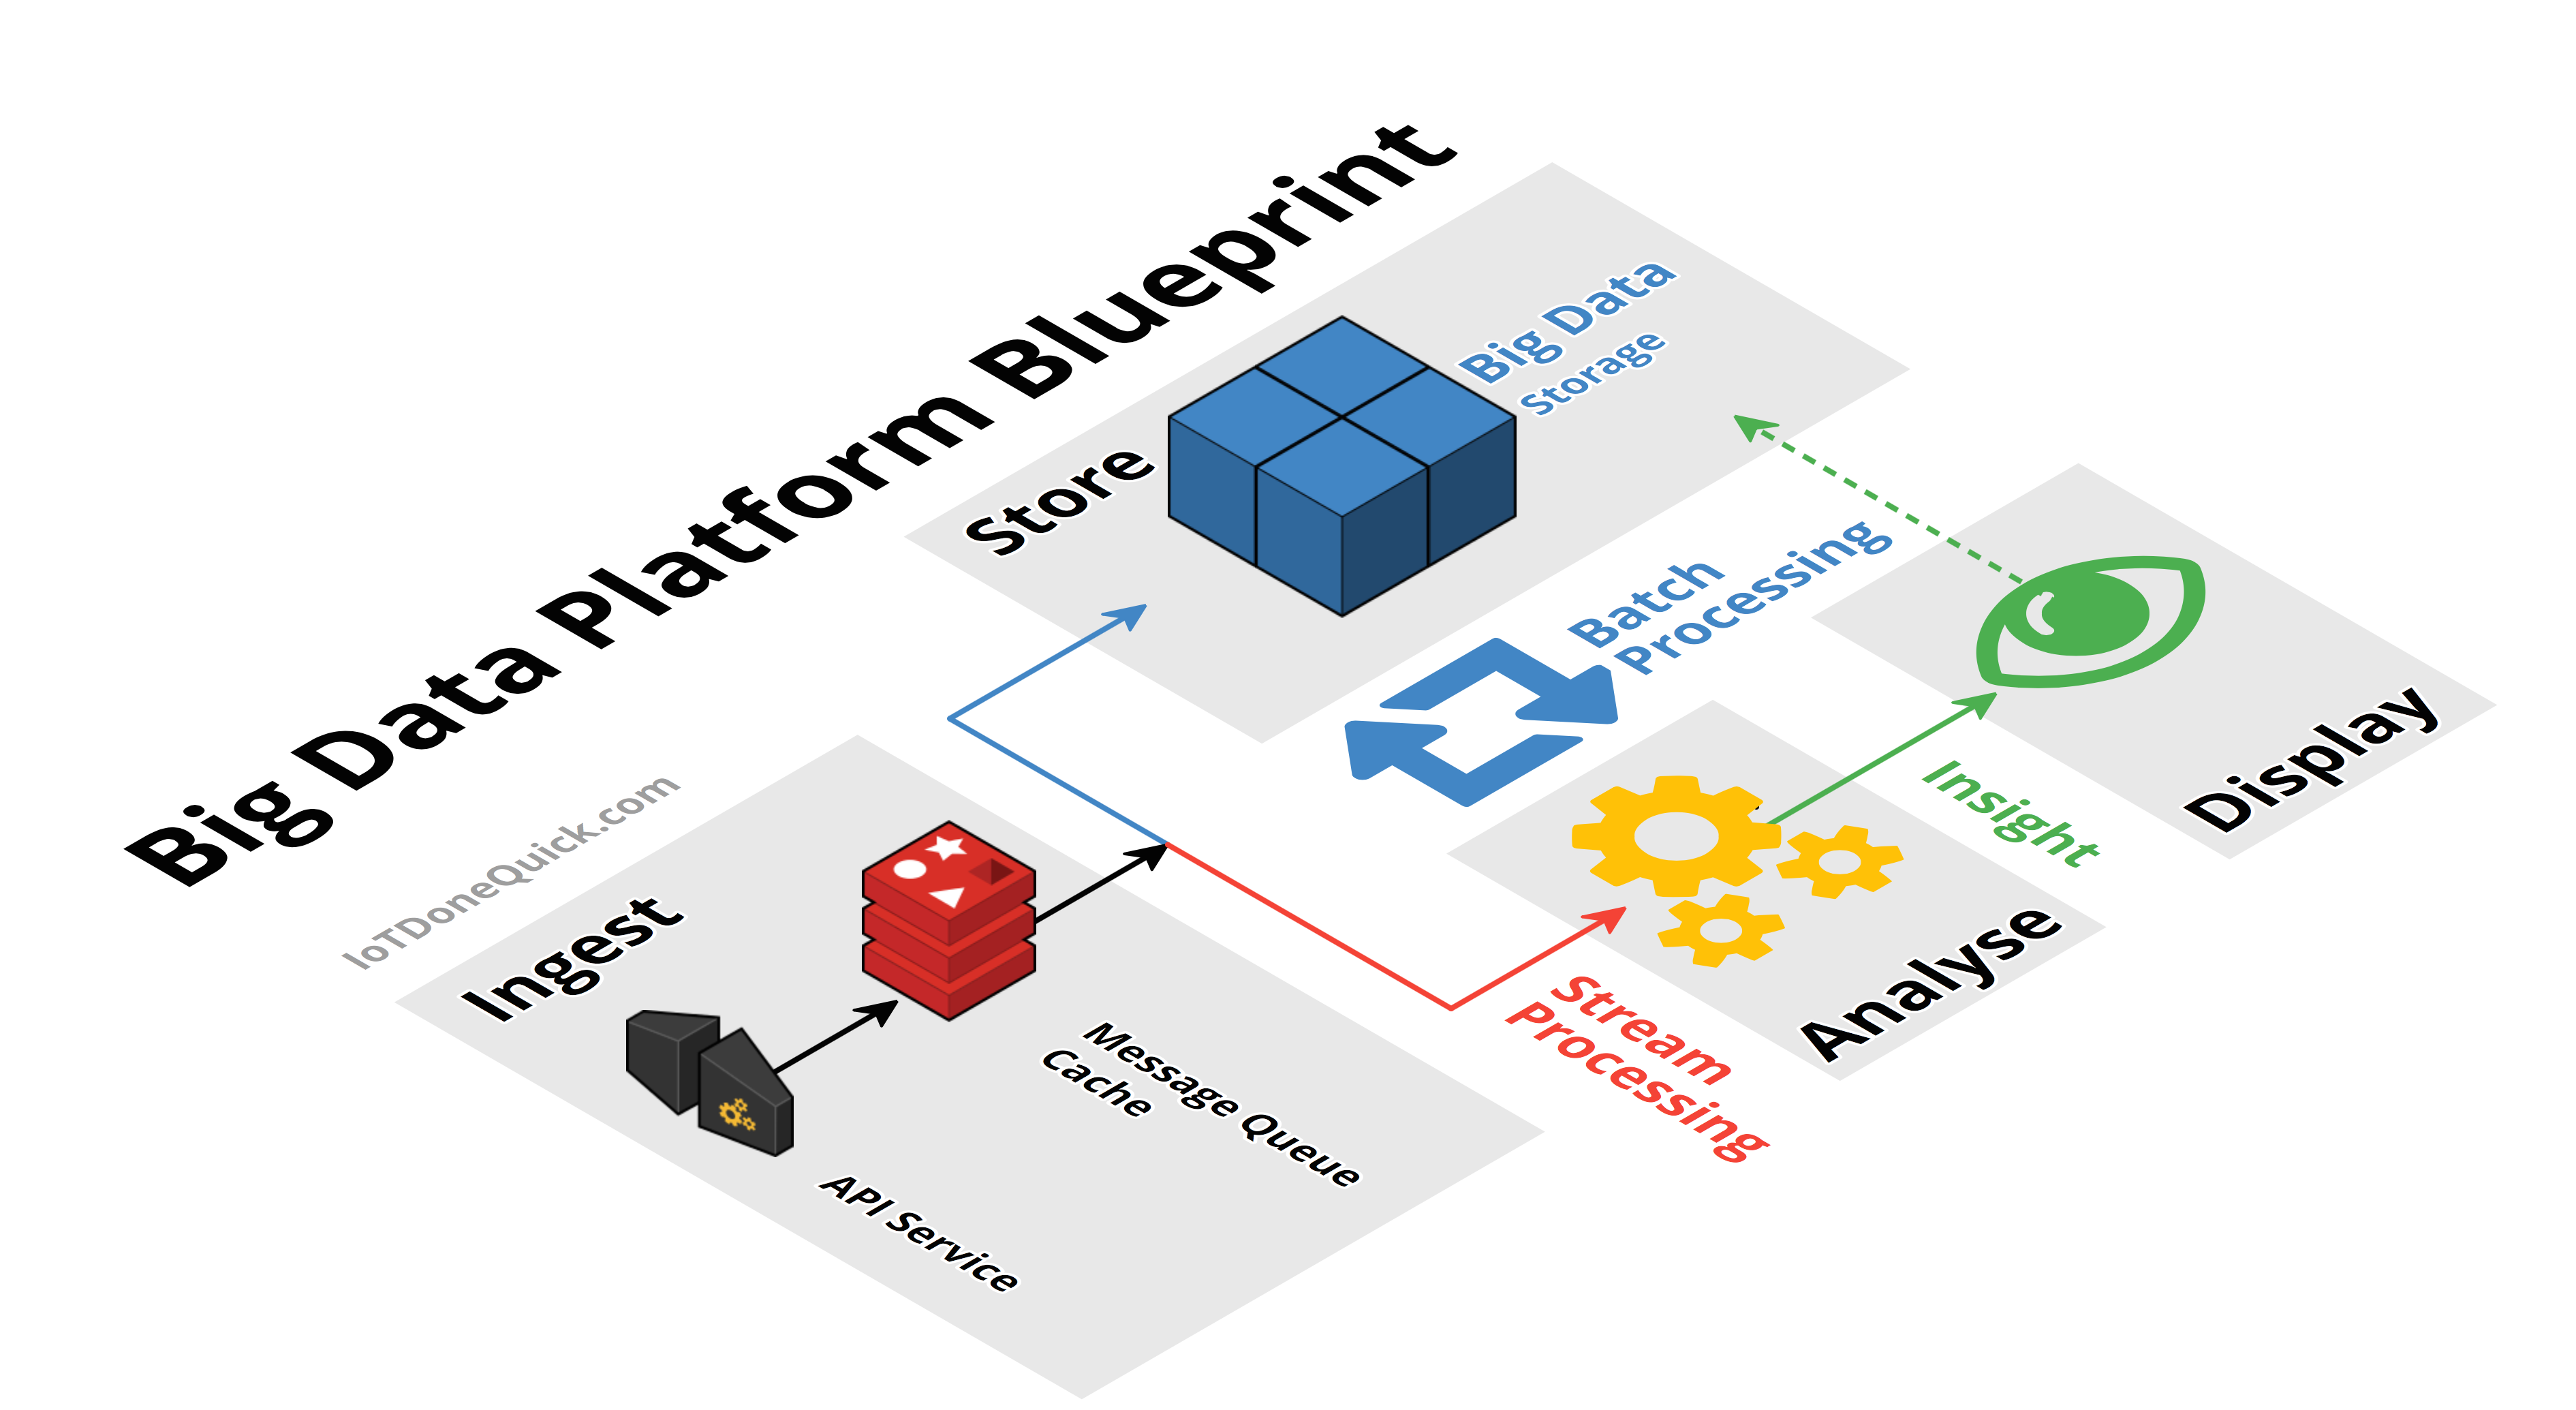
\includegraphics[width=0.9\textwidth]{images/Big-Data-Platform-Blueprint-Title-Original.png}
  \caption{Platfrom Blueprint}
  \label{fig:Bild1}
\end{figure}


Having the platform split like this turns it it a modular platform with loosely coupled interfaces.

Why is it so important to have a modular platform?

If you have a platform that is not modular you end up with something that is fixed or hard to modify. This means you can not adjust the platform to changing requirements of the company.

Because of modularity it is possible to switch out every component, if you need it.

Now, lets talk more about each key area.

\section{Ingest}
Ingestion is all about getting the data in from the source and making it available to later stages. Sources can be everything form tweets, server logs to IoT sensor data like from cars.

Sources send data to your API Services. The API is going to push the data into a temporary storage.

The temporary storage allows other stages simple and fast access to incoming data.

A great solution is to use messaging queue systems like Apache Kafka, RabbitMQ or AWS Kinesis. Sometimes people also use caches for specialised applications like Redis.

A good practice is that the temporary storage follows the publish, subscribe pattern. This way APIs can publish messages and Analytics can quickly consume them.

\section{Analyse / Process}
The analyse stage is where the actual analytics is done. Analytics, in the form of stream and batch processing.

Streaming data is taken from ingest and fed into analytics. Streaming analyses the “live” data thus, so generates fast results.

As the central and most important stage, analytics also has access to the big data storage. Because of that connection, analytics can take a big chunk of data and analyse it.

This type of analysis is called batch processing. It will deliver you answers for the big questions.

To learn more about stream and batch processing read my blog post: How to Create New and Exciting Big Data Aided Products

The analytics process, batch or streaming, is not a one way process. Analytics also can write data back to the big data storage.

Often times writing data back to the storage makes sense. It allows you to combine previous analytics outputs with the raw data.

Analytics insight can give meaning to the raw data when you combine them. This combination will often times allow you to create even more useful insight.

A wide variety of analytics tools are available. Ranging from MapReduce or AWS Elastic MapReduce to Apache Spark and AWS lambda.

\section{Store}
This is the typical big data storage where you just store everything. It enables you to analyse the big picture.

Most of the data might seem useless for now, but it is of upmost importance to keep it. Throwing data away is a big no no.

Why not throw something away when it is useless?

Although it seems useless for now, data scientists can work with the data. They might find new ways to analyse the data and generate valuable insight from it.

What kind of systems can be used to store big data?

Systems like Hadoop HDFS, Hbase, Amazon S3 or DynamoDB are a perfect fit to store big data.

Check out my podcast how to decide between SQL and NoSQL: https://anchor.fm/andreaskayy/embed/episodes/NoSQL-Vs-SQL-How-To-Choose-e12f1o

\section{Display}
Displaying data is as important as ingesting, storing and analysing it. People need to be able to make data driven decisions.

This is why it is important to have a good visual presentation of the data. Sometimes you have a lot of different use cases or projects using the platform.

It might not be possible for you to build the perfect UI that fits everyone. What you should do in this case is enable others to build the perfect UI themselves.

How to do that? By creating APIs to access the data and making them available to developers.

Either way, UI or API the trick is to give the display stage direct access to the data in the big data cluster. This kind of access will allow the developers to use analytics results as well as raw data to build the the perfect application.

\chapter{ Lambda Architecture}

\section{Batch Processing} Ask the big questions. Remember your last yearly tax statement?

You break out the folders. You run around the house searching for the receipts.

All that fun stuff.

When you finally found everything you fill out the form and send it on its way.

Doing the tax statement is a prime example of a batch process.

Data comes in and gets stored, analytics loads the data from storage and creates an output (insight):

\begin{figure}[htbp]
  \centering
     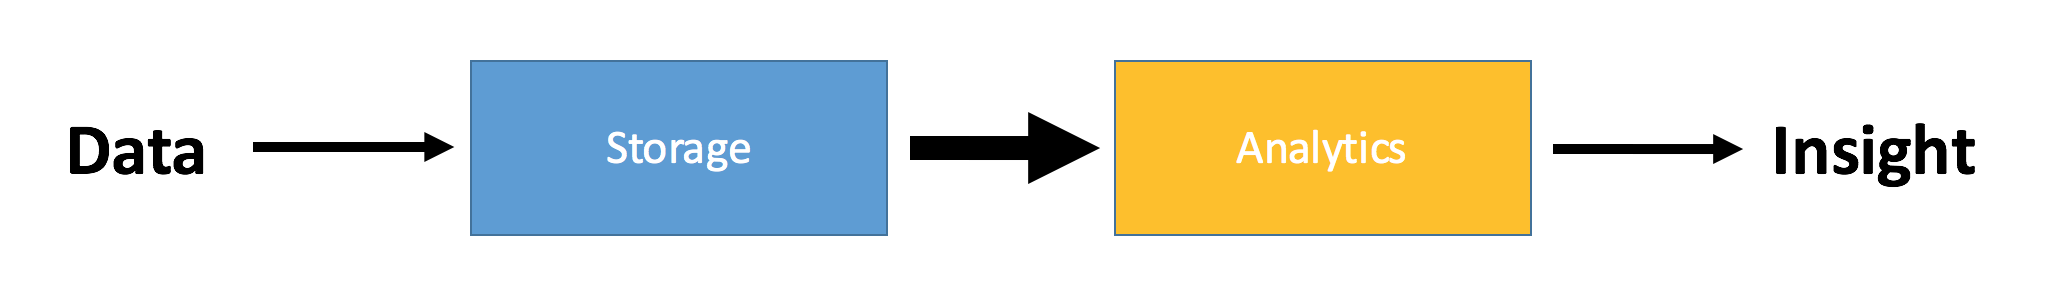
\includegraphics[width=0.9\textwidth]{images/Simple-Batch-Processing-Workflow}
  \caption{Batch Processing Pipeline}
  \label{fig:Bild1}
\end{figure}

Batch processing is something you do either without a schedule or on a schedule (tax statement). It is used to ask the big questions and gain the insights by looking at the big picture.

To do so, batch processing jobs use large amounts of data. This data is provided by storage systems like Hadoop HDFS.

They can store lots of data (petabytes) without a problem.

Results from batch jobs are very useful, but the execution time is high. Because the amount of used data is high.

It can take minutes or sometimes hours until you get your results.



\section{Stream Processing} Gain instant insight into your data.

Streaming allows users to make quick decisions and take actions based on “real-time” insight. Contrary to batch processing, streaming processes data on the fly, as it comes in.

With streaming you don’t have to wait minutes or hours to get results. You gain instant insight into your data.

In the batch processing pipeline, the analytics was after the data storage. It had access to all the available data.

Stream processing creates insight before the data storage. It has only access to fragments of data as it comes in.

As a result the scope of the produced insight is also limited. Because the big picture is missing.

\begin{figure}[htbp]
  \centering
     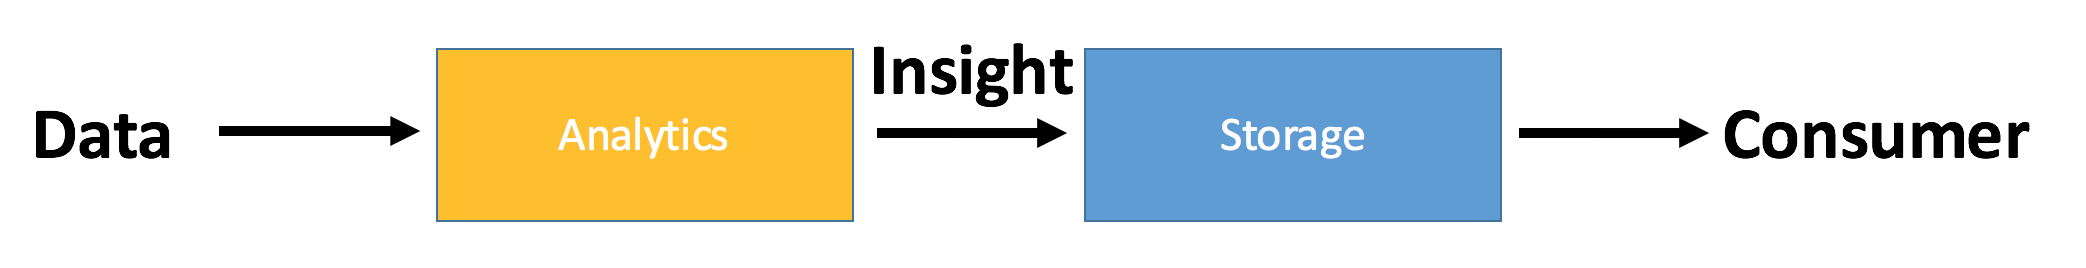
\includegraphics[width=0.9\textwidth]{images/Simple-Stream-Processing-Workflow}
  \caption{Stream Processing Pipeline}
  \label{fig:Bild1}
\end{figure}

Only with streaming analytics you are able to create advanced services for the customer. Netflix for instance incorporated stream processing into Chuckwa V2.0 and the new Keystone pipeline.

One example of advanced services through stream processing is the Netflix “Trending Now” feature.
Check out the Netflix case study.

\section{Should you do stream or batch processing?}

It is a good idea to start with batch processing. Batch processing is the foundation of every good big data platform.

A batch processing architecture is simple, and therefore quick to set up. Platform simplicity means, it will also be relatively cheap to run.

A batch processing platform will enable you to quickly ask the big questions. They will give you invaluable insight into your data and customers.

When the time comes and you also need to do analytics on the fly, then add a streaming pipeline to your batch processing big data platform.


\section{Lambda Architecture Alternative }
\subsection{Kappa Architecture}
\subsection{Kappa Architecture with Kudu}

\chapter(What We Want To Do)

\begin{itemize}
\item Twitter data to predict best time to post using the hashtag datascience or ai
\item Find top tweets for the day
\item Top users
\item Analyze sentiment and keywords
\end{itemize}


\chapter{Thoughts On Choosing The Target Environment}

\section{Cloud vs On-Premise}

\section{Cloud Native or Independent Vendors}

\chapter{Thoughts On Choosing A Development Environment}

\section{Cloud As Dev Environment}

\section{Local Dev Environment}



\section{Data Architecture}

\subsection{Source Data}

\subsection{Analytics Requirements For Streaming}

\subsection{Analytics Requirements For Batch Processing}

\subsection{Data Visualization}

\section{Milestone 1 | Tool Decisions}










\part{Case Studies}

\chapter{How I do Case Studies}

\section{Data Science @Airbnb}
\url{https://medium.com/airbnb-engineering/airbnb-engineering-infrastructure/home}

Airbnb Engineering Blog:
\url{https://medium.com/airbnb-engineering}

Data Infrastructure:
\url{https://medium.com/airbnb-engineering/data-infrastructure-at-airbnb-8adfb34f169c}

Scaling the serving tier:
\url{https://medium.com/airbnb-engineering/unlocking-horizontal-scalability-in-our-web-serving-tier-d907449cdbcf}

Druid Analytics:
\url{https://medium.com/airbnb-engineering/druid-airbnb-data-platform-601c312f2a4c}

Spark Streaming for logging events:
\url{https://medium.com/airbnb-engineering/scaling-spark-streaming-for-logging-event-ingestion-4a03141d135d}

-Druid Wiki:
\url{https://en.wikipedia.org/wiki/Apache_Druid}

\subsection{Data Science @Amazon}
\url{https://www.datasciencecentral.com/profiles/blogs/20-data-science-systems-used-by-amazon-to-operate-its-business} \\
\url{https://aws.amazon.com/solutions/case-studies/amazon-migration-analytics/}

\section{Data Science @Baidu}
\url{https://www.slideshare.net/databricks/spark-sql-adaptive-execution-unleashes-the-power-of-cluster-in-large-scale-with-chenzhao-guo-and-carson-wang}

\section{Data Science @Blackrock}
\url{https://www.slideshare.net/DataStax/maintaining-consistency-across-data-centers-randy-fradin-blackrock-cassandra-summit-2016}

\section{Data Science @BMW}
Big Data in der Automobilindustrie – Daten aus dem Fahrzeug nutzen \url{https://www.unibw.de/code.../ws3_bigdata_vortrag_widmann.pdf}

\section{Data Science @Booking.com}
\url{https://www.slideshare.net/ConfluentInc/data-streaming-ecosystem-management-at-bookingcom?ref=https://www.confluent.io/kafka-summit-sf18/data-streaming-ecosystem-management}

\url{https://www.slideshare.net/SparkSummit/productionizing-behavioural-features-for-machine-learning-with-apache-spark-streaming-with-ben-teeuwen-and-roman-studenikin}

\url{https://www.slideshare.net/ConfluentInc/data-streaming-ecosystem-management-at-bookingcom?ref=https://www.confluent.io/kafka-summit-sf18/data-streaming-ecosystem-management}

Druid:
\url{https://towardsdatascience.com/introduction-to-druid-4bf285b92b5a}

Kafka Architecture:
\url{https://data-flair.training/blogs/kafka-architecture/}

Confluent Platform:
\url{https://www.confluent.io/product/confluent-platform/}


\section{Data Science @CERN}
\url{https://en.wikipedia.org/wiki/Large_Hadron_Collider}

\url{http://www.lhc-facts.ch/index.php?page=datenverarbeitung}

\url{https://openlab.cern/sites/openlab.web.cern.ch/files/2018-09/2017_ESADE_Madrid_Big_Data.pdf}

\url{https://openlab.cern/sites/openlab.web.cern.ch/files/2018-05/kubeconeurope2018-cern-180507122303.pdf}

\url{https://www.slideshare.net/SparkSummit/next-cern-accelerator-logging-service-with-jakub-wozniak}

\url{https://databricks.com/session/the-architecture-of-the-next-cern-accelerator-logging-service}

\url{http://opendata.cern.ch}

\url{https://gobblin.apache.org}

\url{https://www.slideshare.net/databricks/cerns-next-generation-data-analysis-platform-with-apache-spark-with-enric-tejedor}

\url{https://www.slideshare.net/SparkSummit/realtime-detection-of-anomalies-in-the-database-infrastructure-using-apache-spark-with-daniel-lanza-and-prasanth-kothuri}


\section{Data Science @Disney}
\url{https://medium.com/disney-streaming/delivering-data-in-real-time-via-auto-scaling-kinesis-streams-72a0236b2cd9}

\section{Data Science @Drivetribe}
\url{https://berlin-2017.flink-forward.org/kb_sessions/drivetribes-kappa-architecture-with-apache-flink/}

\url{https://www.slideshare.net/FlinkForward/flink-forward-berlin-2017-aris-kyriakos-koliopoulos-drivetribes-kappa-architecture-with-apache-flink}

\section{Data Science @Dropbox}
\url{https://blogs.dropbox.com/tech/2019/01/finding-kafkas-throughput-limit-in-dropbox-infrastructure/}

\section{Data Science @Ebay}
\url{https://www.slideshare.net/databricks/moving-ebays-data-warehouse-over-to-apache-spark-spark-as-core-etl-platform-at-ebay-with-kim-curtis-and-brian-knauss}
\url{https://www.slideshare.net/databricks/analytical-dbms-to-apache-spark-auto-migration-framework-with-edward-zhang-and-lipeng-zhu}

\section{Data Science @Expedia}
\url{https://www.slideshare.net/BrandonOBrien/spark-streaming-kafka-best-practices-w-brandon-obrien}
\url{https://www.slideshare.net/Naveen1914/brandon-obrien-streamingdata}

\section{Data Science @Facebook}
\url{https://code.fb.com/core-data/apache-spark-scale-a-60-tb-production-use-case/}

\subsection{Data Science @Google}		
\url{http://www.unofficialgoogledatascience.com/} \\		
\url{https://ai.google/research/teams/ai-fundamentals-applications/} \\		
\url{https://cloud.google.com/solutions/big-data/} \\		
\url{https://datafloq.com/read/google-applies-big-data-infographic/385}

\section{Data Science @@Grammarly}
\url{https://www.slideshare.net/databricks/building-a-versatile-analytics-pipeline-on-top-of-apache-spark-with-mikhail-chernetsov}

\section{Data Science @ING Fraud}
\url{https://sf-2017.flink-forward.org/kb_sessions/streaming-models-how-ing-adds-models-at-runtime-to-catch-fraudsters/}

\section{Data Science @Instagram}
\url{https://www.slideshare.net/SparkSummit/lessons-learned-developing-and-managing-massive-300tb-apache-spark-pipelines-in-production-with-brandon-carl}

\section{Data Science @LinkedIn}
\url{https://engineering.linkedin.com/teams/data#0}

\url{http://www.bigdatausecases.info/companies/linkedin}

\section{Data Science @Lyft}
\url{https://eng.lyft.com/running-apache-airflow-at-lyft-6e53bb8fccff}

\section{Data Science @NASA}
\url{http://sites.nationalacademies.org/cs/groups/ssbsite/documents/webpage/ssb_182893.pdf}

\url{https://esip.figshare.com/articles/Apache_Science_Data_Analytics_Platform/5786421}

\url{http://www.socallinuxexpo.org/sites/default/files/presentations/OnSightCloudArchitecture-scale14x.pdf}

\url{https://www.slideshare.net/SparkSummit/spark-at-nasajplchris-mattmann?qid=90968554-288e-454a-b63a-21a45cfc897d&v=&b=&from_search=4}

\url{https://en.m.wikipedia.org/wiki/Hierarchical_Data_Format}

\section{Data Science @Netflix -- available}

Netflix revolutionized how we watch movies and tv. Currently over 75 million users watch 125 million hours of Netflix content every day!

Netflix’s revenue comes from a monthly subscription service. So, the goal for Netflix is to keep you subscribed and to get new subscribers.

To achieve this, Netflix is licensing movies from studios as well as creating its own original movies and tv series.

But offering new content is not everything. What is also very important is, to keep you watching content that already exists.

To be able to recommend you content, Netflix is collecting data from users. And it is collecting a lot.

Currently, Netflix analyses about 500 billion user events per day. That results in a stunning 1.3 petabytes every day.

All this data allows Netflix to build recommender systems for you. The recommenders are showing you content that you might like, based on your viewing habits, or what is currently trending.

\paragraph{The Netflix batch processing pipeline}
When Netflix started out, they had a very simple batch processing system architecture.

The key components were Chuckwa, a scalable data collection system, Amazon S3 and Elastic MapReduce.

\begin{figure}[htbp]
  \centering
     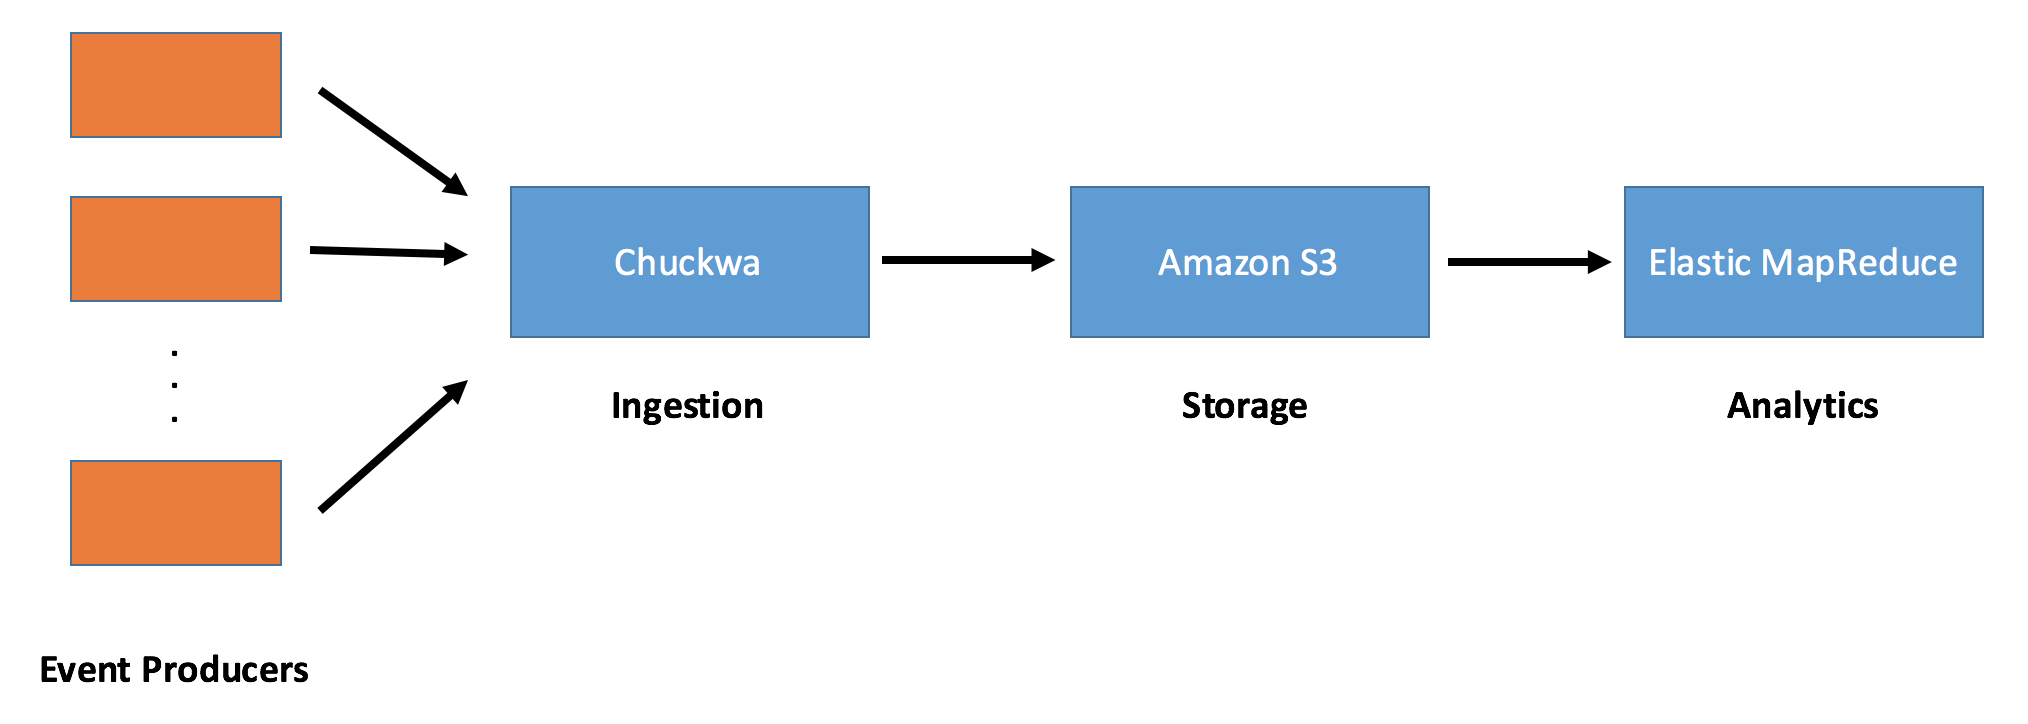
\includegraphics[width=0.9\textwidth]{images/Netflix-Chuckwa-Pipeline}
  \caption{Old Netflix Batch Processing Pipeline}
  \label{fig:Bild1}
\end{figure}

Chuckwa wrote incoming messages into Hadoop sequence files, stored in Amazon S3. These files then could be analysed by Elastic MapReduce jobs.

Netflix batch processing pipeline
Jobs were executed regularly on a daily and hourly basis. As a result, Netflix could learn how people used the services every hour or once a day.

\paragraph{Know what customers want:}

Because you are looking at the big picture you can create new products. Netflix uses insight from big data to create new tv shows and movies.

They created House of Cards based on data. There is a very interesting Ted talk about this you should watch:

How to use data to make a hit TV show | Sebastian Wernicke:


Batch processing also helps Netflix to know the exact episode of a TV show that gets you hooked. Not only globally but for every country where Netflix is available.

Check out the article from TheVerge

They know exactly what show works in what country and what show does not.

It helps them create shows that work in everywhere or select the shows to license in different countries. Germany for instance does not have the full library that Americans have :(

We have to put up with only a small portion of tv shows and movies. If you have to select, why not select those that work best.

\paragraph{Batch processing is not enough}

As a data platform for generating insight the Cuckwa pipeline was a good start. It is very important to be able to create hourly and daily aggregated views for user behavior.

To this day Netflix is still doing a lot of batch processing jobs.

The only problem is: With batch processing you are basically looking into the past.

For Netflix, and data driven companies in general, looking into the past is not enough. They want a live view of what is happening.

\paragraph{The trending now feature}
One of the newer Netflix features is “Trending now”. To the average user it looks like that “Trending Now” means currently most watched.

This is what I get displayed as trending while I am writing this on a Saturday morning at 8:00 in Germany. But it is so much more.

What is currently being watched is only a part of the data that is used to generate “Trending Now”.

\begin{figure}[htbp]
  \centering
     
\includegraphics[width=0.9\textwidth]{images/Netflix-Trending-Now-Screenshot}
  \caption{Netflix Trending Now Feature}
  \label{fig:Bild1}
\end{figure}

“Trending now” is created based on two types of data sources: Play events and Impression events.

What messages those two types actually include is not really communicated by Netflix. I did some research on the Netflix Techblog and this is what I found out:

Play events include what title you have watched last, where you did stop watching, where you used the 30s rewind and others.
Impression events are collected as you browse the Netflix Library like scroll up and down, scroll left or right, click on a movie and so on

Basically, play events log what you do while you are watching. Impression events are capturing what you do on Netflix, while you are not watching something.

\paragraph{Netflix real-time streaming architecture}
Netflix uses three internet facing services to exchange data with the client’s browser or mobile app. These services are simple Apache Tomcat based web services.

The service for receiving play events is called “Viewing History”. Impression events are collected with the “Beacon” service.

The “Recommender Service” makes recommendations based on trend data available for clients.

Messages from the Beacon and Viewing History services are put into Apache Kafka.
It acts as a buffer between the data services and the analytics.

Beacon and Viewing History publish messages to Kafka topics. The analytics subscribes to the topics and gets the messages automatically delivered in a first in first out fashion.

After the analytics the workflow is straight forward. The trending data is stored in a Cassandra Key-Value store. The recommender service has access to Cassandra and is making the data available to the Netflix client.

\begin{figure}[htbp]
  \centering
     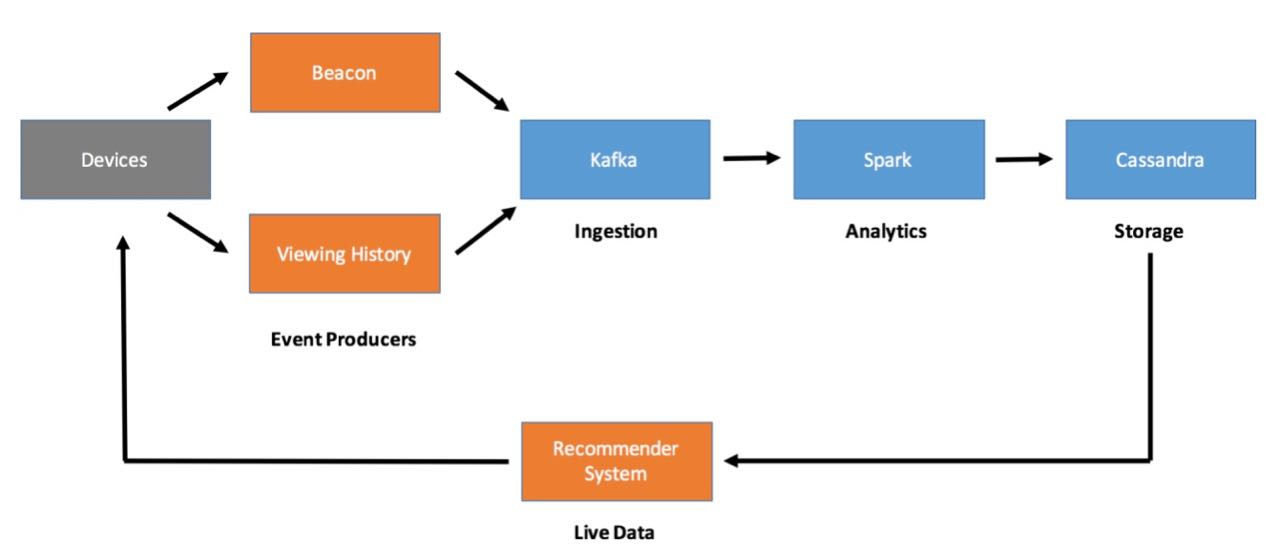
\includegraphics[width=0.9\textwidth]{images/Netflix-Streaming-Pipeline}
  \caption{Netflix Streaming Pipeline}
  \label{fig:Bild1}
\end{figure}


The algorithms how the analytics system is processing all this data is not known to the public. It is a trade secret of Netflix.

What is known, is the analytics tool they use. Back in Feb. 2015 they wrote in the tech blog that they use a custom made tool.

They also stated, that Netflix is going to replace the custom made analytics tool with Apache Spark streaming in the future. My guess is, that they did the switch to Spark some time ago, because their post is more than a year old.

\section{Data Science @OLX}

\begin{table}[h]
\begin{tabular}{ll}
\hline
\multicolumn{2}{l}{\textbf{Podcast Episode:} \#083 Data Engineering at OLX Case Study} \\ \hline
\multicolumn{2}{p{15cm}}{This podcast is a case study about OLX with Senior Data Scientist Alexey Grigorev as guest. It was super fun.}         \\ \hline
\multicolumn{1}{l|}{Audio}     & \href{https://anchor.fm/andreaskayy/episodes/083-Data-Engineering-at-OLX-Case-Study-e45j5n}{Click here to listen}   \\
\multicolumn{1}{l|}{Youtube}   & \href{https://youtu.be/H_uFNoCvykM}{Click here to watch}   \\ \hline
\end{tabular}
\end{table}

\textbf{Slides:}

\url{https://www.slideshare.net/mobile/AlexeyGrigorev/image-models-infrastructure-at-olx}




\section{Data Science @OTTO}
\url{https://www.slideshare.net/SparkSummit/spark-summit-eu-talk-by-sebastian-schroeder-and-ralf-sigmund}

\section{Data Science @Paypal}
\url{https://www.paypal-engineering.com/tag/data/}

\section{Data Science @Pinterest}
\textbf{Slides:}

\url{https://www.slideshare.net/ConfluentInc/pinterests-story-of-streaming-hundreds-of-terabytes-of-pins-from-mysql-to-s3hadoop-continuously?ref=https://www.confluent.io/kafka-summit-sf18/pinterests-story-of-streaming-hundreds-of-terabytes} 

\url{https://www.slideshare.net/ConfluentInc/building-pinterest-realtime-ads-platform-using-kafka-streams?ref=https://www.confluent.io/kafka-summit-sf18/building-pinterest-real-time-ads-platform-using-kafka-streams}

\url{https://medium.com/@Pinterest_Engineering/building-a-real-time-user-action-counting-system-for-ads-88a60d9c9a}

\url{https://medium.com/pinterest-engineering/goku-building-a-scalable-and-high-performant-time-series-database-system-a8ff5758a181}

\url{https://medium.com/pinterest-engineering/building-a-dynamic-and-responsive-pinterest-7d410e99f0a9}

\url{https://medium.com/@Pinterest_Engineering/building-pin-stats-25ec8460e924}

\url{https://medium.com/@Pinterest_Engineering/improving-hbase-backup-efficiency-at-pinterest-86159da4b954}

\url{https://medium.com/@Pinterest_Engineering/pinterest-joins-the-cloud-native-computing-foundation-e3b3e66cb4f}

\url{https://medium.com/@Pinterest_Engineering/using-kafka-streams-api-for-predictive-budgeting-9f58d206c996}

\url{https://medium.com/@Pinterest_Engineering/auto-scaling-pinterest-df1d2beb4d64}

\section{Data Science @Salesforce}
\url{https://engineering.salesforce.com/building-a-scalable-event-pipeline-with-heroku-and-salesforce-2549cb20ce06}

\section{Data Science @Slack}
\url{https://speakerdeck.com/vananth22/streaming-data-pipelines-at-slack}

\section{Data Science @Spotify}
\url{https://labs.spotify.com/2016/02/25/spotifys-event-delivery-the-road-to-the-cloud-part-i/}

\url{https://www.slideshare.net/InfoQ/scaling-the-data-infrastructure-spotify}

\section{Data Science @Symantec}
\url{https://www.slideshare.net/planetcassandra/symantec-cassandra-data-modelling-techniques-in-action}

\section{Data Science @Tinder}
\url{https://www.slideshare.net/databricks/scalable-monitoring-using-apache-spark-and-friends-with-utkarsh-bhatnagar}

\section{Data Science @Twitter}
\url{https://www.slideshare.net/sawjd/real-time-processing-using-twitter-heron-by-karthik-ramasamy}

\url{https://www.slideshare.net/sawjd/big-data-day-la-2016-big-data-track-twitter-heron-scale-karthik-ramasamy-engineering-manager-twitter}

\section{Data Science @Uber}
\url{https://eng.uber.com/uber-big-data-platform/}

\url{https://eng.uber.com/aresdb/}

\url{https://www.uber.com/us/en/uberai/}

\section{Data Science @Upwork}
\url{https://www.slideshare.net/databricks/how-to-rebuild-an-endtoend-ml-pipeline-with-databricks-and-upwork-with-thanh-tran}

\section{Data Science @Woot}
\url{https://aws.amazon.com/de/blogs/big-data/our-data-lake-story-how-woot-com-built-a-serverless-data-lake-on-aws/}

\section{Data Science @Zalando}
\url{https://jobs.zalando.com/tech/blog/what-is-hardcore-data-science--in-practice/?gh_src=4n3gxh1}

\url{https://jobs.zalando.com/tech/blog/complex-event-generation-for-business-process-monitoring-using-apache-flink/}


\newpage

\begin{thebibliography}{99}

\bibitem{einstein}
J.~Ely and I.~Stavrov,
\emph{Analyzing chalk dust and writing speeds: computational and geometric approaches},
BoDine Journal of Mathematics \textbf{3} (2001), 14-159.

\end{thebibliography}


\listoffigures% Abbildungsverzeichnis
% \listoftables% Tabellenverzeichnis

\end{document}
